\documentclass{article}

\usepackage[spanish]{babel}
\usepackage{amsmath}
\usepackage{amssymb}
\usepackage[a4paper]{geometry}
\usepackage{parskip}
\usepackage[document]{ragged2e} %para alinear el texo 
\usepackage[utf8]{inputenc}
\usepackage{graphicx}
\usepackage[T1]{fontenc}
\graphicspath{ {imagenes/} }
\usepackage{xcolor}
\usepackage{multirow} % para las tablas
\usepackage{wrapfig} % para poner texto en tablas
\usepackage[nottoc]{tocbibind} %Adds "References" to the table of contents
\usepackage{tikz}
\usetikzlibrary{babel}

\usepackage{hyperref} % para que los titulos me lleven al sitio que toca 
\usepackage{url} % para la biblio para poner web

\usepackage{multicol} % para hacer columas con el texto



\newcommand{\RomanNumeralCaps}[1]
    {\MakeUppercase{\romannumeral #1}}

\title{\Huge \textbf{Criptografía}}
\author{Marina Fabregat Expósito}
\date{}

\begin{document}


 % \maketitle

\begin{titlepage}
\centering
{\scshape \LARGE Colegio Sant Josep Obrer \par}
%\vspace{1cm}
%{\scshape \Large  \par}
\vspace{1.5cm}
{\huge \bfseries Criptografía y \TeX \par}
\vspace{2cm}



\vfill % todo lo que ponga después se va para abajo
{\Large \itshape Marina Fabregat Expósito \par}

Tutor: Artur Arroyo \\

2019-2020

\end{titlepage}


%        \begin{center}
%           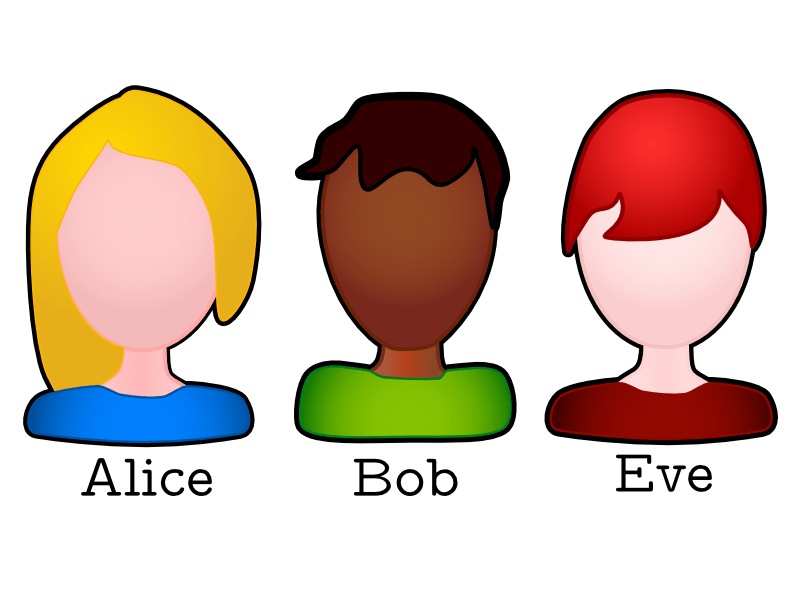
\includegraphics[scale=0.3]{portada.png} 
%        \end{center}


\vfill

\begin{abstract}
\justify
Aquest treball de recerca tracta diversos aspectes del món de la criptografia. Primer explicaré l'evolució dels sistemes criptogràfics al llarg de la història, des del xifrat Cèsar fins al xifrat de Vernam. 
 
Després es veurà reflexada la comprensió d'aquestes idees al marc pràctic, on es troben una sèrie d'excercisis. En aquestes activitats he utilitzat gairebé tots els conceptes mencionats al marc teòric. A més he fet una exaltació del programa TEX. Explico com he utilitzat aquest, amb exemples i breus explicacions. 
 

 
 \vspace{10mm} %5mm vertical space
 \justify
 This research project addresses vairous aspects of the world of cryptography. Firstly, I will epxlain the evolution of cryptography systems troughout history, from Cesar encrypted to Vernam encrypted.
 
 The understanding of this ideas will be reflected in the practical framework, where are a serie of exercices. In these activities I have used almost all the concepts mentioned in the theorical framework. I also had done an exaltation of the TEX program. I had explanied how I used it, with examples and brief explanations.
 
\end{abstract}

\newpage
\tableofcontents
\newpage



\centering \textbf{\large Introducción}
\justify
Desde la antigüedad todas las civilizaciones han desarrollado sistemas de criptografía para que las comunicaciones no fueran públicas. Aunque antiguamente y a lo largo de toda su historia la criptografía ha sido utilizada como una de las armas intelectuales más potentes en el campo militar. Los sistemas de encriptación han acelerado su desarrollo, sobretodo en la primera (Maquina Enigma) y la segunda guerra mundial, desde finales del siglo \RomanNumeralCaps{20}. Esta técnica o ciencia es fundamental para proporcionar privacidad en las comunicaciones que utilizamos en la vida diaria. Asimismo hoy en día muchas personas utilizan lenguajes específicos para que solamente los iniciados en ellos puedan comprender la conversación como, por ejemplo, las jergas utilizadas en ambientes carcelarios. 

La seguridad en las redes siempre ha sido un tema importante y gracias a la criptografía se pueden garantizar las propiedades de integridad y confidencialidad, pero hay que saber cómo utilizarla. Para ello es importante tener claros los conceptos básicos que están detrás de los sistemas criptográficos modernos. En el siguiente trabajo vamos a abordar diferentes conceptos de la criptografía. En primer lugar se presentará una definición, seguido de una clasificación histórica de esta ciencia. 

He elegido este tema porque, entre otras ideas que me llaman la atención dentro de la informática, la seguridad en la red es algo que me impresionó. También quería profundizar mis conocimientos en este mundo, ya que partía de una base limitada. Al mismo tiempo he seleccionado este tema de entre muchos otros porque me gustaría enfocar mi carrera profesional en ello. Y lo considero una pequeña introducción de lo que me gustaría profundizar en el ámbito académico y profesional. 

%En cuanto a la motivación que me ha ayudado mucho a seguir con este trabajo es la de extender mi conocimiento.  

Para este proyecto he utilizado una serie de materiales que me han proporcionado lo necesario para obtener mi objetivo. Entre estos encontramos todo tipo de páginas web que me han guiado a la hora de buscar información útil y compararla con mis conocimientos. Primero me he decidido por extraer toda la información posible para ir encontrando la más adecuada para mi trabajo. Después la he ordenado y la he redactado de la forma más clara posible para una buena comprensión del texto. También me he ayudado de los conceptos que adquirí en un curso \footnote{UPF, Univeristat Pompeu Fabra, curso de ``Hackers Matemáticos en la Red'' un total de 25 horas.} que asistí en verano del 2019, donde me hicieron una pequeña introducción en el mundo de la criptografía. En este curso, me explicaron diferentes métodos de cifra y aclararon todo tipo de dudas.



Para realizar este trabajo he partido de dos hipótesis diferentes pero relacionadas entre ellas:

En primer lugar, es verificar si soy capaz de aprender a utilizar \LaTeX. \LaTeX \; es un sistema de composición de textos, orientado a documentos que presentan una alta calidad tipográfica. Normalmente usado a nivel mundial en los ámbitos universitario y científico. Su creador Donald Knuth, desarrolló este sistema de manera que todo el mundo pueda utilizarlo y aportar mejoras a este. He decidido trabajar con este sistema y no con cualquier otro como podría ser el Word o Google Docs, por la utilidad de sus funciones para redactar formulas matemáticas. El trabajo que he desarrollado con \LaTeX \; queda explicado al final del documento con una serie de indicaciones básicas de su funcionamiento.

Y en segundo lugar comprobar que sí que puedo llegar a comprender los diferentes métodos de criptografía clásica. Se verificara o no esta hipótesis con el marco práctico, con toda una serie de ejercicios que incluyen operaciones y cálculos que se explican en el marco teórico. He decido hablar de este mundo de la informática, porque como he mencionado al principio me gustaría enfocarme en este campo en mi futuro ámbito académico y a ser posible profesional también.

\newpage

\section{Definición de criptografía}
\justify
Etimológicamente la palabra \emph{Criptografía} viene del griego $\kappa \rho \upsilon \pi \tau \sigma \varsigma$, \emph{Kryptos}, escondido, y \emph{Graphos}, escritura. Es decir, cuando se habla de Criptografía se habla de ``escritura escondida''. Se trata de escribir algo de manera que otra persona que quiera leer el mensaje no pueda entenderlo a no ser que conozca cómo se ha escondido. Dicho de otra manera, la criptografía se ha definido como el ámbito de la criptología que se ocupa de las técnicas de cifrado o codificado destinadas a alterar las representaciones lingüísticas de ciertos mensajes con el fin de hacerlos ininteligibles a receptores no autorizados. 

Por consiguiente, el principal objetivo que tenía la criptografía era conseguir la confidencialidad de los mensajes, para lo cual se diseñaban sistemas de cifrado y códigos, y la única criptografía existente era la llamada criptografía clásica. 

\section{Clasificación histórica de criptosistemas}
\justify
La clasificación actual de los sistemas de cifra se basa en el tratamiento de la información (cifrado en bloque o cifrado en flujo) o bien en el tipo de clave que se utiliza en la cifra (sistemas de clave secreta o sistemas de clave pública), pero según su relación con la historia de la criptografía podríamos clasificarlos como: 
\begin{center}
    \textbf{Sistemas de Cifra Clásicos versus Sistemas de Cifra Modernos} 
\end{center}
\justify
Esta no es la mejor clasificación desde el punto de vista de la ingeniería y la informática pero permitirá comprobar el desarrollo de estas técnicas de la cifra desde una perspectiva histórica. Además, nos permitirá criptoanalizar con cierta facilidad prácticamente todos estos sistemas y comprobar también las teorías de Shannon \footnote{Esta teoría está relacionada con las leyes matemáticas que rigen la transmisión y el procesamiento de al información y se ocupa de la medición de la información y de la representación de la misma, así como también de la capacidad de los sistemas de comunicación para transmitir y procesar información.} sobre las estadísticas del lenguaje. 


\section{Herramientas de la criptografía clásica}
\justify
Tanto máquinas, artilugios de cifra, como los algoritmos que trabajan matemáticamente dentro de un cuerpo finito n, hacen uso de dos técnicas básicas orientadas a caracteres y que, muchos siglos después, las propondrá Shannon como herramientas para fortalecer la cifra. La definición es la siguiente y más adelante se desarrollaran:
\justify
 
\begin{itemize}
    \item \textbf{Técnicas de transposición o permutación} Se basa en que los caracteres o letras del mensaje en claro se redistribuyen sin modificarlos y según unas reglas, dentro del criptograma. El criptograma tendrá entonces los mismos caracteres del mensaje en claro pero con una distribución o localización diferente.
    \item \textbf{Técnicas de sustitución} Se basa en que los caracteres o letras del mensaje en claro se modifican o sustituyen por otros elementos o letras en la cifra. El criptograma tendrá entonces caracteres distintos a los que tenía el mensaje claro. 
\end{itemize}
\newpage
%       AÑADIR EJEMPLOS O ALGO ....

\section{Cifrado por transposición}
\subsection{Escítala}
\justify
La escítala era usada en el siglo \RomanNumeralCaps{5} a.C. por el pueblo griego de los lacedemonios. Consistía en un bastón en el que se enrollaba una cinta de cuero y luego se escribía en ella el mensaje de forma longitudinal. Al desenrollar la cinta, las letras aparecerán desordenadas. 

Para descifrar el criptograma y recuperar el mensaje en claro habrá que enrollar dicha cinta en un bastón con el mismo diámetro que el usado en el extremo emisor y leer el mensaje de forma longitudinal. La clave del sistema se encuentra en el \textsl{diámetro} del bastón. Dicho de otra manera, en ese bastón residía la fortaleza de un pueblo. Por ello, y como símbolo de poder, el bastón de mando que se le entrega al alcalde de una ciudad en la ceremonia de su nombramiento, proviene de estos tiempos tan remotos. 

Se trata de una cifra por transportación puesto que los caracteres del criptograma son los mismos que en el texto en claro pero están distribuidos de otra forma dentro del criptograma. 


\begin{center}
   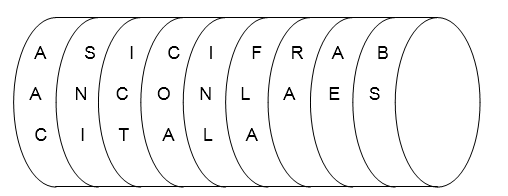
\includegraphics[scale=0.5]{escitala} 
\end{center}

El texto en claro o ``\emph{M}'' es:
\begin{center}
    \texttt{ASI CIFRABAN CON LA ESCITALA}
\end{center}

El texto cifrado, criptograma o ``\emph{C}'' será:

\begin{center}
    \texttt{AAC SNI ICT COA INL FLA RA AE BS}
\end{center}

\section{Cifrado por sustitución}
\subsection{Polybios}
\justify

El algoritmo de Polybios es el cifrado por sustitución de caracteres más antiguo que se conoce (siglo \RomanNumeralCaps{2} a.D) i por lo tanto, es el primer cifrado por sustitución de caracteres. Recibe el nombre Polybios en reconocimiento al historiador griego del mismo nombre y de quien se considera que fue su creador. Este cifrado consiste en sustituir un carácter por el número o letra de una columna o fila. El inconveniente es que como duplica el tamaño de texto en claro, con letras o números, no fue tan buena idea al no ser del todo útil.

El algoritmo Polybios \cite{1} puede utilizar como base de cifrado una de las dos tablas de sustitución siguientes:


 \begin{table}[htbp]
\begin{tabular}{c|ccccc}

 & A & B & C & D & E \\ \hline
A & A & B & C & D & E \\
B & F & G & H & I/J & K \\ 
C & L & M & N & O & P\\
D & Q & R & S & T & U \\ 
E & V & W & X & Y  & Z\\

\end{tabular}
%\caption{}%
\end{table}


\begin{table}[htbp]
\begin{tabular}{c|ccccc}

 & 1 & 2 & 3 & 4 & 5 \\ \hline
1 & A & B & C & D & E \\
2 & F & G & H & I/J & K \\ 
3 & L & M & N & O & P\\
4 & Q & R & S & T & U \\ 
5 & V & W & X & Y  & Z\\

\end{tabular}
%\caption{}%
\end{table}


Para llevar a cabo el proceso de cifrado se considera la primera columna y el primer renglón de una de las tablas anteriores como el par criptográfico correspondiente a cada letra dentro de la matriz 5x5 mostradas en las tablas. De manera que justo en ese orden, renglón-columna, son las dos letras que sustituyen a cada una de las letras que se pueden conformar el mensaje en claro. 

Por ejemplo el mensaje en claro M = \emph{QUE BUENA IDEA}, pasaría a ser C= \emph{DA DE AE AB DE AE CC AA BD AD AE EA}.

%Al mismo tiempo el mensaje en claro M =\emph{LA DEL GRIEGO}, pasaría a ser C= 31 11 14 15 31 22 42 24 15 22 34.

%\begin{center}
%    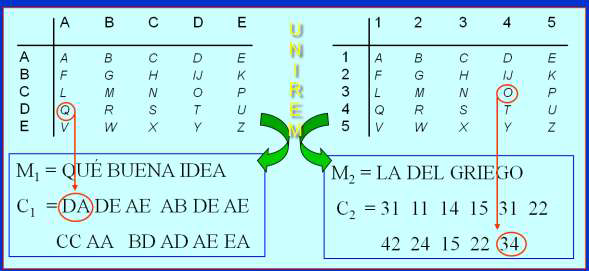
\includegraphics[scale=0.5]{polybios.png} 
%\end{center}

\subsection{El cifrado del César}
\justify
El cifrado del César es uno de los primeros y más simples de los cifrados por sustitución. De aquí deriva la mayor parte de la criptografía actual. En el siglo \RomanNumeralCaps{1} a.D., Julio César ya usaba este cifrado, es por eso por lo que se le atribuye su nombre al método de cifrado.

El algoritmo consiste en el desplazamiento de tres espacios hacia la derecha de los caracteres del texto en claro. Es un cifrado por sustitución monoalfabético en el que las operaciones se realizan módulo $n$, siendo $n$ el número de elementos del alfabeto (en aquel entonces el latín). El alfabeto de cifrado del César para castellano es de $mod \; 27$.

Cada letra se cifrará siempre igual. Esto es una gran debilidad y hace que este sistema sea muy vulnerable y fácil de atacar, simplemente usando las estadísticas del lenguaje.
\begin{equation*}
\begin{split}
    \text{Cifrado:}  \; C_{i} & =(M_{i}+b)\; mod \; 27 \\
    \text{Descifrado:}\; M_{i} & =(C_{i}-b)\; mod \;27 
\end{split}
\end{equation*}




\subsubsection{Ejemplo de cifra del César en mod 27 }

Cifrado: $C_{i}=M{i}+3 \; mod \;27$ 

Descifrado: $M_{i}=C_{i}-3 \;mod \;27$

%$M_i =\quad$A B C D E F G H I J K L M N Ñ O P Q R S T U V W X Y Z 

%$C_i =\quad$D E F G H I J K L M N Ñ O P Q R S T U V W X Y Z A B C

%\begin{center}
%    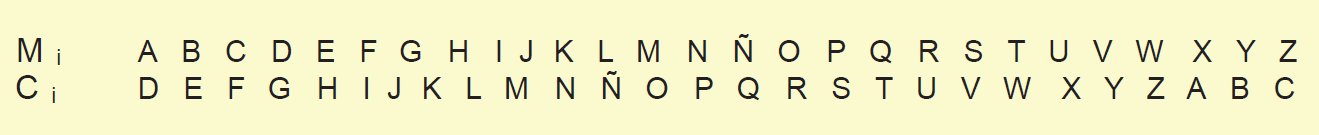
\includegraphics[scale=0.4]{cesarr.png} 
%\end{center}



$M=$ EL PATIO DE MI CASA ES PARTICULAR 

$C=$ H\~N SDWLR GH OL FDVD HV SDUWLFX\~NDU

\subsubsection{Criptoanálisis del cifrador por sustitución}
\justify

Para atacar el mensaje cifrado, se encuentra la letra más frecuente del criptograma se hace coincidir con la más frecuente del lenguaje, que en este caso es el castellano, la letra E, y se encuentra así $b$. 

Si el mensaje cifrado es:
C= \emph{LZAHL ZBTHW YBLIH XBLKL ILYOH ZLYCH ROKH} 

Las frecuencias observadas en el criptograma son: L(7); H(6); Z(3); B(3); Y(3); I (2); K(2); O(2); A(1); T(1); W(1); X(1); C(1); R(1). 

Es posible que la letra E del lenguaje se cifre como L. Comprobamos además si la letra A (la segunda más frecuente) se cifra como H:

$E+b \; mod \; 27=L\Rightarrow b=L-E \; mod \; 27 = 11-4\; mod \; 27= 7$

$A+b \; mod\;27=H \Rightarrow b=H-A \; mod \; 27=7-0\;mod\; 27=7 $

M$=$ ESTA ES UNA PRUEBA QUE DEBERÍA SER VALIDA

\subsection{Cifrado por sustitución afín mod 27}
\begin{equation*}
\begin{split}
    \text{Cifrado:}  \; C_{i}&=a*M_{i}+b\; mod \; 27 \\
    \text{Descifrado:}\; M_{i}&=\left ( C_{i}-b \right ) * a^{-1}\; mod \; 27 \quad \text{Donde:} \; a^{-1}=inv\left ( a,27 \right )
\end{split}
\end{equation*}

Para utilizar este tipo de cifrado hay que tener en cuenta los siguientes factores:
\begin{itemize}
    \item El factor de multiplicación $a$ deberá ser primo relativo con el cuerpo $n$ (en este caso 27) para que exista el inverso $a^{-1}$
    \item El factor de desplazamiento puede ser cualquiera: $0\leq b \leq 26$.
\end{itemize}
\justify
El ataque a este sistema es también muy elemental. Se relaciona el elemento más frecuente del criptograma a la letra E y el segundo a la letra A, planteando un sistema de 2 ecuaciones. Si el texto tiene varias decenas de caracteres este ataque prospera; caso contrario, podría haber ligeros cambios en esta distribución de frecuencias.

\subsubsection{Criptoanálisis a la cifra afín mod 27}

C= \emph{ NAQÑF EKNDP NCIVU FPUAN EJUIP FCNER NFRÑF UNPLN\newline
    AFPFQ TFPEI JRTÑE FPKÑI KTAPF LIKIÑ AIPÑU RCUJI\newline
    PCIVU CUNER IRLNP TJIAF NEOIÑ CFLNC NLUFA TEF}

Los caracteres más frecuentes en el criptograma son: F = 14; N = 13; I = 12

Con E y A las más frecuentes, el ataque falla. En un segundo intento se supone la letra A más frecuente que la E:

$ F = \left(a*A+B\right) mod \thinspace 27 \Rightarrow  \left(a*0+B\right) mod \thinspace 27 = 5 \Rightarrow b=5$
$F = \left(a*E+B\right) mod \thinspace 27 \Rightarrow  \left(a*4+B\right) mod \thinspace 27 = 13$

Entonces $a= \left(13-5\right) * inv \left(4, 27\right) mod \thinspace 27 = 8 * 7 mod \thinspace 27 =2$

$C_{i}= \left(2*M_{i}+5\right) mod \thinspace 27 \Rightarrow M_{i}= \left(C_{i}-5\right)*inv\left(2,27\right) = \left(C_{i}-5\right)*14 mod \thinspace 27 $
\justify
M= El gran pez se movía silenciosamente a través de las aguas nocturnas, propulsado por los rítmicos movimientos de su cola en forma de media luna. 
(Comienzo de la novela "Tiburón" de \textit{Peter Bencchley})

\subsection{El cifrado de Vigenère}
\justify
Lo que ahora se conoce como el cifrado Vigenère, fue originalmente descrito por Giovan Battista Belasso en su libro \emph{La cifra del Sig. Giovan Battista Belasso}, en 1533. Este cifrado polialfabético soluciona la debilidad del cifrado del César en que una letra se cifra siempre igual. Es decir, es un cifrado basado en diferentes series de caracteres o letras del cifrado César formando estos caracteres una tabla, llamada Vigenère. Se usa una clave K de longitud L y se cifra carácter a carácter sumando módulo $n$ al texto en claro con los elementos de esta clave. 

\begin{equation*}
        C_{i}= M_{i} + K_{i}\; mod \; 27
\end{equation*}

Sea K = \emph{CIFRA} y el mensaje M= \emph{HOLA AMIGOS}

%
%
% ALGUNA TABLA O ALGOASIIII 
%
%

\subsubsection{¿Es Vigenère un algoritmo seguro?}
\justify
Si la clave de Vigenère tiene más de 6 caracteres distintos, se logra una distribución de frecuencias en el criptograma del tipo normal, es decir más o menos plana, por lo que se logra difuminar la redundancia del lenguaje. 
Aunque pudiera parecer que usando una clave larga y de muchos caracteres distintos, y por lo tanto varios alfabetos de cifrado, Vigenère es un sistema de cifra seguro, esto es falso. 
La redundancia del lenguaje unido a técnicas de criptoanálisis muy sencillas, como los métodos de Kasiki y del Índice de Coincidencia, permiten romper la cifra y la clave de una manera muy fácil y con mínimos recursos. 

\subsubsection{Ataque por el método de Kasiski}
\justify
Públicado en 1863 por un oficial prusiano, Friedrich Kasiski. El método de Kasiski consiste en buscar repeticiones de cadenas de caracteres en el criptograma. Si estas cadenas son mayores o iguales a tres caracteres y se repiten más de una vez, lo más probable es que esto se deba a cadenas típicas del texto en claro (trigramas, tetragramas, etc., muy comunes) que se han cifrado con una misma porción de la clave. 

Si se detectan estas cadenas, la distancia entre las mismas será múltiplo de la longitud de la clave. Luego, el máximo común divisor entre esas cadenas es un candidato a ser la longitud de la clave, digamos L.

Dividimos el criptograma en L subcriptogramas que entonces han sido cifrados por una misma letra de la clave y en cada subcripyograma hacemos un ataque simple ahora de tipo estadistíco monoalfabético. 

La idea es buscar ahora a través de los tres caracteres más frecuentes en cada subcriptograma las posiciones relativas de las letras A, E y O que en castellano están sepradas por 4 y 11 espacios. La letra de la posición que ocupe la letra A $\left(A=0\right)$ será entonces la letra clave correspondiente. 
\justify
\footnotesize

PBVRQ \ VICAD \ SKAÑS \ DETSJ \ PSIED \ B\textcolor{red}{GGMP} \ SLRPW \ RÑPW\textcolor{red}{Y} \ \textcolor{red}{EDS}DE \ ÑDRDP \ CRCPQ \ MNPWK \\
UBZVS \ FNVRD \ MTIPW \ UEQVV \ CBOVN \ UEDIF \ QLONM \ WNUVR \ SEIKA \ ZYEAC \ E\textcolor{red}{YEDS} \ ETFPH \\
LBHGU \ ÑESOM \ EHLBX \ VAEEP \ UÑELI \ SEVEF \ WHUNM \ CLPQP \ MBRRN \ BPVIÑ \ MTIBV \ VEÑID \\
ANSJA \ MTJOK \ MDODS \ ELPWI \ UFZOM \ QMVNF \ O\textcolor{red}{HASE} \ SRJWR \ SFQCO\ TWVMB \ JGRPW \ \textcolor{red}{VSUE}X \\
INQRS \ JEUEM \ GGRBD \ GNNIL \ AGSJI \ DS\textcolor{red}{VSU} \ \textcolor{red}{E}EINT \ GRUEE \ TF\textcolor{red}{GGM} \ \textcolor{red}{P}ORDF \ OGTSS \ TOSEQ\\
OÑTGR \ RYVLP \ WJIFW \ XOTGG \ RPQRR \ JSKET \ XRNBL \ ZETGG \ NEMUO \ TXJAT \ ORVJH \ RSFHV \\
NUEJI \ BC\textcolor{red}{HAS} \ \textcolor{red}{E}HEUE \ UOTIE \ FFGYA \ T\textcolor{red}{GGMP} \ IKTBW \ UEÑEN \ IEEU.
 


%\begin{center}
%    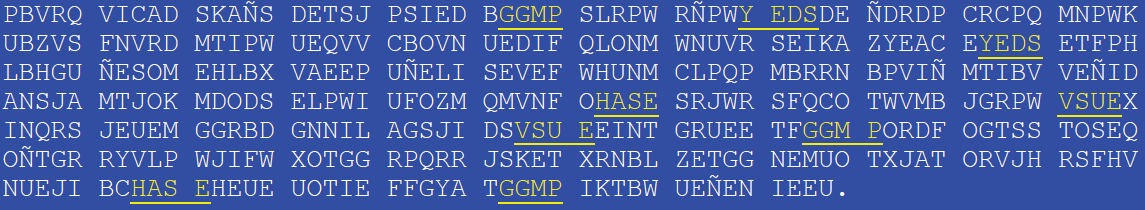
\includegraphics[scale=0.45]{ataquekasiski.png} 
%\end{center}
\normalsize
Entre otras, se observan las siguientes cadenas (subrayadas) en el criptograma: 
\begin{center}
    3 cadenas GGMP, separadas por 256 y 104  posiciones. \\
    2 cadenas YEDS, separadas por 72 espacios.\\
    2 cadenas HASE, separadas por 156 espacios.\\
    2 cadenas, separadas por 32 espacios
\end{center}
\justify
Luego el período de la clave puede ser mcd $(256, 104, 72, 156, 32) = 4$. La clave tendrá cuatro caracteres, por lo tanto tomaremos del criptograma el carácter número 1, el 5, el 9, etc para formar el primer subcriptograma $C_{A}$; luego el segundo, el sexto, el décimo, etc para formar el subcriptograma $C_{B}$, y lo mismo para subcriptogramas $C_{C}$ y $C_{C}$.
Tenemos ahora 4 subcriptogramas de sólo 101 letras c/u (muy importante tenerlo en cuenta en las estadísticas) que han sido cifrados con la misma letra de la clave.  

%\begin{center}
%    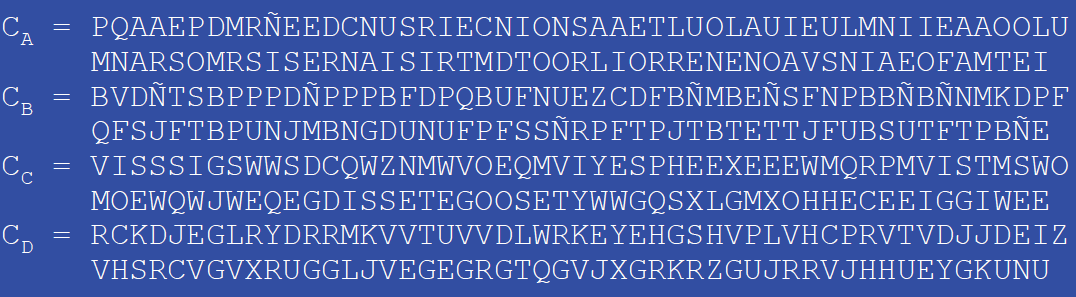
\includegraphics[scale=0.45]{AK1.png} 
%\end{center}

$C_{A}=$ PQAAEPDMRÑEEDCNUSRIECNIONSAAETLUOLAUIEULMNIIEAAOOLUMNARSOMRSISERNAISIRTMDTOORLIORRENENOAVSNIAEOFAMTEI

$C_{B}=$ BVDÑTSBPPPDÑPPPBFDPQBUFNUEZCDFBÑMBEÑSFNPBBÑBÑNMKDPFQFSJETBPUNJNMBNGDUNUFPFSSÑRPETPJTBTETTJFUBSUTFTPBÑE

$C_{C}=$ VISSSIGSWWSDCQWZNMWVOEQMVIYESPHEEXEEEWMQRPMVISTMSWOMO
EWQWJWEQEGDISSETEGOOSETYWWGQSXLGMXOHHECEEIGGIWEE

$C_{D}=$ RCKDJEGLRYDRRMKVVTUVVDLWRKEYEHGSHVPLVHCPRVTVDJJDEIZVHSR
CVGVXRUGGLJVEGEGRGTQGVJXGRKRZGUJRRVJHHUEYGKUNU


La frecuencia relativa observada en cada uno de los subcriptogramas es:
\

\begin{table}[htbp]

\tabcolsep=0.11cm %espacio entre columnas

\begin{tabular}{l|lllllllllllllllllllllllllll}
 

 & A & B & C & D & E & F & G & H & I & J & K & L & M & N  & Ñ & O & P & Q & R & S & T & U & V & W & X & Y & Z \\ \hline
 $C_A$ & 12 & 0 & 2 & 3 & 12 & 1 & 0 & 0 & 11 & 0 & 0 & 5 & 6 & 9 & 1 & 10 & 2 & 1 & 9 & 7 & 4 & 5 & 1 & 0 & 0 & 0 & 0\\
 $C_B$ & 0 & 14 & 1 & 6 & 4 & 15 & 1 & 0 & 0 & 4 & 1 & 0 & 3 & 6 & 8 & 0 & 14 & 2 & 1 & 6 & 9 & 7 & 1 & 0 & 0 & 0 & 1\\
 $C_C$ & 0 & 0 & 2 & 2 & 18 & 0 & 7 & 3 & 7 & 1 & 0 & 1 & 7 & 1 & 0 & 6 & 2 & 6 & 1 & 12 & 3 & 0 & 4 & 12 & 3 & 2 & 1 \\
 $C_D$ & 0 & 0 & 3 & 5 & 7 & 0 & 12 & 6 & 1 & 7 & 5 & 4 & 1 & 1 & 0 & 0 & 2 & 1 & 13 & 2 & 3 & 6 & 14 & 1 & 2 & 3 & 2\\
 
\end{tabular}
%\caption{}
\label{tabla:sencilla}

\end{table}


%\begin{center}
%    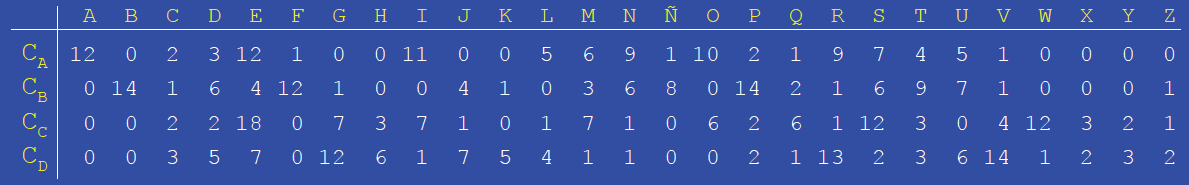
\includegraphics[scale=0.45]{AK2.png} 
%\end{center}

Luego, la letra más frecuente del subcriptograma debería corresponder a la letra E del texto en claro, La segunda a la letra A y la tercera a la letra O.

\textsl{\large La regla AEO en el ataque de Kasiski}

\begin{itemize}
    \item Si la posición relativa de la letra \textcolor{red}{A} es el valor 0, entonces la letra E está cuatro espacios a la derecha de A ($m+4 mod \thinspace 27 $) y la letra O está 15 espacios a la derecha de A ($m+ 15 mod \thinspace 27 $) y a 11 de la letra E.
    \item Buscaremos en cada subcriptograma $C_{i}$ las tres letras más frecuentes que cumplan además con esa distribución: $0\rightarrow +4 \rightarrow +11 mod \thinspace 27$.
    \item Es suficiente contar con estas tres letras para que el ataque prospere. No obstante, podemos afinar un poco más el ataque si tomamos en cuenta la siguiente letra frecuente en el castellano, S, en la posición ($m+19$) $mod \thinspace 27$.
\end{itemize}
\justify
En el ejemplo para $C_{A}$ se observa que la única solución que cumple con esto es la que coincide la AEO (12, 12, 10) luego la letra clave sería la A. Para $C_{B}$ elegimos BFP (14, 12, 14) por lo que la letra clave sería B. Para $C_{C}$ elegimos EIS (18, 7, 12) por lo que la letra clave sería E. Para $C_{D}$ elegimos RVG (13, 14, 12) por lo que la letra clave sería R.

Con la clave $K=ABER$ obtenemos "Para que la cosa no me sorprenda..." Al ser éste un texto largo y con sentido, hemos encontrado la clave. 
\subsubsection{El índice de coincidencia IC}
%\textbf{\textsl{\large El índice de coincidencia IC}}
\justify
El estudio del índice IC queda fuera del contexto de los apuntes. Si bien bien tiene relación con el número de alfabetos, no es efectivo como Kasiski.






Si el IC es menor que 0,5 es muy probable que no se trate de un cifrador monoalfabético sino polialfabético con un periodo 2 o mayor.
Así, cuando encontramos una longitud L se la clave por el método de Kasiski y rompemos el criptograma en L subcriptogramas, aplicando el concepto del índice de coincidencia IC podemos comprobar que cada uno de ellos se trata efectivamente de un cifrado monoalfabético cuando para cada subcriptograma este valor se acerca a 0,072 o lo supera.
En el ejemplo anterior, una vez roto el criptograma en cuatro tenemos: \\ 
$IC_{CA}=0,080; IC_{CB}=0,091; IC_{CC}=0,083; IC_{CD}=0,082...$

\subsection{Cifrador poligrámico de Playfair}
\justify
Los cifrados anteriores se hacían carácter a carácter, es decir eran monográmicos. Para aumentar la seguridad de la cifra y romper las estadísticas, podemos cifrar por poligramas, bloques de caracteres. 

Un cifrador inventado a finales del siglo \RomanNumeralCaps{19} es el de Playfair que trabaja con una matriz de $5x5$ letras, cifrando por digramas. Si el texto en claro tiene un número impar de elementos se rellena una letra preestablecida, por ejemplo la letra X.

\begin{table}[htbp]
\begin{tabular}{|l|l|l|l|l|}
\hline 
A & B & C & D & E \\ \hline
F & G & H & I/J & K \\ \hline
L & M & N/Ñ & O & P \\ \hline
Q & R & S & T & U \\ \hline
V & W & X & Y & Z \\ 
\hline
\end{tabular}
%\caption{}%
\label{tabla:sencilla}

\end{table}

\begin{itemize}
    \item Si $M_{1}M_{2}$ están en la misma fila, $C_{1}C_{2}$ son los dos caracteres de la derecha.
    \item Si $M_{1}M_{2}$ están en la misma columna,  $C_{1}C_{2}$ son los dos caracteres de abajo.
    \item Sii $M_{1}M_{2}$ están en filas y columnas distintas, $C_{1}C_{2}$ son los dos caracteres de la diagonal, desde la fila de $M_{1}$.
\end{itemize}

\subsubsection{Ejemplo de cifra con Playfair}

%\textbf{\textsl{\large Ejemplo de cifra con Playfair}}

Si la clave $K=$ BEATLES y eliminamos la letra Ñ (inglés), ciframos el mensaje $M=$ WITH A LITTLE HELP FROM MY FRIENDS. 

\begin{table}[htbp]
\begin{tabular}{|l|l|l|l|l|}
\hline 
B & E & A & T & L \\ \hline
S & C & D & F & G \\ \hline
H & I/J & K & M & N \\ \hline
O & P & Q & R & U \\ \hline
V & W & X & Y & Z \\ 
\hline
\end{tabular}
%\caption{}%
\end{table}

Se rompe la doble MM agregando una X y se rellena al final también con X.
 
M $=$ WI TH AL IT TL EH EL PF RO MX MY FR IE ND SX

C $=$ EP BM TB ME LB BI AB RC UP KY RT MY PC KG DV
\justify
Estos sistemas también son criptoanalizables pues en el criptograma C persisten algunas propiedades del lenguaje; en este caso la distribución de digramas típicos; por ejemplo en el castellano en, de, mb, etc


\subsection{El cifrador de matrices de Hill}
\justify
En 1929 el matemático Lester Hill propone un sistema de cifra usando una matriz como clave, cifrando Ngramas de forma que: 

\begin{equation*}
    \left(
    \begin{array}{c}
    C_1  \\
    C_2  \\
    C_3  \\
    \ldots \\
    C_N 
    \end{array} \right) = \left(
    \begin{array}{ccccc}
    K_{11} & k_{12} & K_{13} & \ldots & K_{NN}  \\
    K_{21} & K_{22} & K_{23} & \ldots & K_{NN} \\ 
     K_{31} & K_{32} & K_{33} & \ldots & K_{NN} \\ 
     \ldots & \ldots & \ldots & & \ldots \\
      K_{N1} & K_{N2} & K_{N3} & \ldots & K_{NN} \\ 
    \end{array}\right)
    \mathbf{X} 
    \left( 
    \begin{array}{c}
    M_1\\
    M_2\\
    M_3\\
    \ldots\\
    M_N
    \end{array} \right) mod \thinspace n
\end{equation*}
\justify

La matriz clave $K$ debe tener inversa $K^{-1}$ en el cuerpo de cifra $n$. Luego, como $K^{-1}=T_{ADJ(K)}/\vert K \vert mod \thinspace n$, en donde $ADJ(K)$ es la matriz adjunta, T es la traspuesta y   $\vert K \vert$  el determinante, este último valor $\vert K \vert$  no podrá ser cero ni tener factores en común con n puesto que está en el denominador (concepto de inverso ya visto). si el texto en claro no es múltiplo del bloque N, se rellena con caracteres predeterminados, por ejemplo la letra X o la Z.

\subsubsection{Ejemplo de cifrado de Hill.}

Sea M = AMIGO CONDUCTOR y la clave K la que se muestra:
\begin{equation*}
    \left(
    \begin{array}{c}
    C_1  \\
    C_2  \\
    C_3 
    \end{array} \right) = \left(
    \begin{array}{ccc}
    16 & 4 & 11\\
    8 & 6 & 18\\
    15 & 19 & 15 
    \end{array}
    \right) \mathbf{X} \left(
    \begin{array}{c}
    0 \\
    12\\
    8
    \end{array}
    \right) mod \thinspace 27
\end{equation*}

K= PELIGROSO será la clave simbólica. Se cifrará el primer trigrama. AMI = 0, 12,8.

M= AMI GOC OND UCT ORZ
$C_{1} = (16*0 + 4*12 + 11*8) mod \thinspace 27 = 136 mod \thinspace 27 = 1 = \textcolor{red}{B} $

$C_{2} = (8*0 + 6*12 + 18*8) mod \thinspace 27= 216 mod \thinspace 27 = 0 = \textcolor{red}{A} $

$C_{3} = (15*0 + 19*12 + 15*8) mod \thinspace 27= 348 mod \thinspace 27 = 24 = \textcolor{red}{X}$
$C = BAX PMA BJE XAF EUM$ (Compruebe Ud. los demás trigramas)

Para descifrar encontramos $K^{-1} = inv (K, 27) = K^{-1} = T_{ADJ(k)} / \vert K \vert mod n$ 
$\vert K \vert = 16 \left(6*15-19*18 \right) + 11 \left( 8*19-15*6 \right) mod \thinspace 27 = 4$ 
\justify
Encontramos luego la matriz adjunta de K, la trasponemos cambiando filas por columnas y la multiplicamos por $inv(\vert K \vert , 27) = (4,27) = 7$ con lo que se obtiene la matriz que se indica. 

\subsubsection{Ejemplo descifrado de Hill}

\begin{equation*}
    \left( \begin{array}{c}
    M 
    \end{array} \right)= \left(
    \begin{array}{c}
    K^{-1}
    \end{array}\right)x
    \left(
    \begin{array}{c}
    C
    \end{array}\right) mod \thinspace n \quad y \quad
    \mathbf{K^{-1}} = \left( \begin{array}{ccc}
    18 & 26 & 15 \\
    24 & 6 & 13 \\
    11 & 24 & 10
    \end{array}   \right)
\end{equation*}
C = \textcolor{red}{BAX} PMA BJE XAF EUM y l a clave $K_{-1}$ es la que se muestra:

\begin{equation*}
    \left(
    \begin{array}{c}
    M_1  \\
    M_2  \\
    M_3 
    \end{array} \right) = \left(
    \begin{array}{ccc}
    18 & 26 & 15\\
    24 & 6 & 13\\
    11 & 24 & 10 
    \end{array}
    \right) \mathbf{X} \left(
    \begin{array}{c}
    1 \\
    0\\
    24
    \end{array}
    \right) mod \thinspace 27
\end{equation*}

Descifrado del primer trigrama del criptograma: $BAX = 1. 0, 24$. 

C= \textcolor{red}{BAX} PMA BJE XAF EUM

$M_1 = (18 * 1 + 26 * 0 + 15 * 24) mod \thinspace 27 = 0 = \textcolor{red}{A}$ \\
$M_2 = (24 * 1 + 6 * 0 + 13 * 24) mod \thinspace 27 = 12 = \textcolor{red}{M}$\\
$M_3 = (11 * 1 + 24 * 0 + 10 * 24) mod \thinspace 27 = 8 = \textcolor{red}{I}$\\

M = AMI GOC OND UCT ORZ

\subsubsection{¿Es seguro el cifrado de Hill?}
\justify
Si con el sistema de Hill se cifran bloques de 8 caracteres, incluso en un cuerpo tan pequeño como $n = 7$ el espacio de claves aumenta de forma espectacular, comparable con DES.

Si el módulo de cifra es un primo $p$, entonces el número de claves válidas es cercano al máximo posible: $p^{x}$ donde $x=d^{2}$, con  $d$ el tamaño de N-grama o de la matriz clave.

No obstante, el sistema no es seguro. Debido a su linealidad será muy fácil hacer un ataque con texto claro conocido según el método de Gauss-Jordan y encontrar así la matriz clave $K$. 

Esto es debido a que aparecen los llamados vectores unitarios en el criptograma o en el texto en claro, o bien se obtienen aplicando este método. 

\subsubsection{Ataque al cifrado de Hill por Gauss0-ordan}
\justify
El método consiste en escribir una matriz 2N-grámica con los elementos del texto en claro y los elementos del criptograma. En esta matriz se realizan operaciones lineales (multiplicar filas por un número y restar filas entre sí) con el objetivo de obtener los vectores unitarios.

Por ejemplo se puede romper la matriz clave K teniendo:

$M = ENU NLU GAR DEL AMA NCH ADE CUY ONO \ldots$\\
$C = \textcolor{red}{WVX IDQ DDO ITQ JGO GJI YMG FVC U}$\textcolor{red}{\~{N}}$ \textcolor{red}{T \ldots}$

\begin{equation*}
    \left( \begin{array}{cccccc}
    E & N & U & \textcolor{red}{W} & \textcolor{red}{V} & \textcolor{red}{X} \\
    N & L & U & \textcolor{red}{I} & \textcolor{red}{D} & \textcolor{red}{Q} \\
    G & A & R & \textcolor{red}{D} & \textcolor{red}{D} & \textcolor{red}{O} \\
    D & E & L & \textcolor{red}{I} & \textcolor{red}{T} & \textcolor{red}{Q} \\
    A & M & A & \textcolor{red}{J} & \textcolor{red}{G} & \textcolor{red}{O} \\
    N & C & H & \textcolor{red}{G} & \textcolor{red}{J} & \textcolor{red}{I} \\
    A & D & E & \textcolor{red}{Y} & \textcolor{red}{M} & \textcolor{red}{G} \\
    C & U & Y & \textcolor{red}{F} & \textcolor{red}{V} & \textcolor{red}{C} \\
    O & N & O & \textcolor{red}{U} & \textcolor{red}{\text{\textit{Ñ}}} & \textcolor{red}{T} 
    \end{array} \right) = \left(     \begin{array}{cccccc}
    4 & 13 & 21 & 23 & 22 & 24 \\
    13 & 11 & 21 & 8 & 3 & 17 \\
    6 & 0 & 18 & 3 & 3 & 15 \\
    3 & 4 & 11 & 8 & 20 & 17 \\
    0 & 12 & 0 & 9 & 6 & 15 \\
    13 & 2 & 7 & 6 & 9 & 8 \\
    0 & 3 & 4 & 25 & 12 & 6 \\
    2 & 21 & 25 & 5 & 22 & 2 \\
    15 & 13 & 15 & 21 & 14 & 20 \\
    \end{array} \right) 
\end{equation*}
\justify

Se deja en la primera columna un número uno en la fila primera y todas las demás filas un cero. Luego se multiplica el vector $(\textcolor{red}{4} 13 21 22 23 24)$ por el $inv (\textcolor{red}{4},27)=7$. Así se obtiene $7 (4 13 21 23 22 24) mod \thinspace 27 = (1 10 12 26 19 6)$. Si esto no se puede hacer con la primera fila movemos los vectores. Hecho esto se va restando las filas respecto de esta primera como se indica:

\begin{equation*}
    \left(     \begin{array}{cccccc}
    4 & 13 & 21 & 23 & 22 & 24 \\
    13 & 11 & 21 & 8 & 3 & 17 \\
    6 & 0 & 18 & 3 & 3 & 15 \\
    3 & 4 & 11 & 8 & 20 & 17 \\
    0 & 12 & 0 & 9 & 6 & 15 \\
    13 & 2 & 7 & 6 & 9 & 8 \\
    0 & 3 & 4 & 25 & 12 & 6 \\
    2 & 21 & 25 & 5 & 22 & 2 \\
    15 & 13 & 15 & 21 & 14 & 20 \\
    \end{array} \right) 
\end{equation*}

\begin{enumerate}
    \item[a)] $2^{a}$ fila $ = 2^a fila - 13 *1^a$ fila $ mod \thinspace  27$
    \item[b)] $3^{a} $fila$ = 3^a fila - 6 *1^a $fila $ mod \thinspace 27$
    \item[c)] $4^{a} $fila $ = 4^a fila - 3 *1^a $fila $ mod \thinspace 27$
    \item[d)] $5^{a} $fila ya tiene un 0
    \item[e)] $6^{a} $fila $ = 6^a $fila$ - 13 *1^a $fila $  mod \thinspace 27$
    \item[f)] $7^{a} $fila ya tiene un 0
    \item[g)] $8^{a} $fila$ = 8^a $fila$ - 2 *1^a $fila $ mod \thinspace 27$
    \item[h)] $9^{a} $fila$ = 9^a $fila$ - 15 *1^a $fila $  mod \thinspace 27$
\end{enumerate}
\justify
Se repite este procedimiento ahora para algún vector en cuya segunda columna tenga un número con inverso en 27 y lo mismo para la tercera columna, moviendo si es preciso los vectores. 

Como la mitad izquierda de la matriz $2N$ era el texto en claro, la parte derecha de la matriz con vectores unitarios corresponderá a la traspuesta de la clave. 

\begin{equation*}
    \left(     \begin{array}{cccccc}
    1 & 0 & 0 & 2 & 5 & 7\\
    0 & 1 & 0 & 3 & 5 & 8\\
    0 & 0 & 1 & 4 & 6 & 9\\
    0 & 0 & 0 & 0 & 0 & 0\\
    0 & 0 & 0 & 0 & 0 & 0\\
    0 & 0 & 0 & 0 & 0 & 0\\
    0 & 0 & 0 & 0 & 0 & 0\\
    0 & 0 & 0 & 0 & 0 & 0\\
    0 & 0 & 0 & 0 & 0 & 0\\
    \end{array} \right) \Rightarrow \mathbf{K} = \left( \begin{array}{ccc}
    2 & 3 & 4\\
    5 & 5 & 6\\
    7 & 8 & 9\\
    \end{array} \right)
\end{equation*}

%(Comprobar que la clave es la utilizada en este cifrado)%

\subsection{El cifrado de Vernam}
\justify
En 1917 Gilbert Vernam propone un cifrador por sustitución binaria con clave de un solo uso (one-time pad) basado en el código Baudot de 5 bits:
\begin{itemize}
    \item[-] La operación de cifra es la función XOR.
    \item[-] Usa una secuencia cifrante binaria y aleatoria $S$ que se obtiene a partir de una clave secreta $K$ compartida por emisor y receptor. 
    \item[-] El algoritmo de descifrado es igual al de cifrado por la involución de la función XOR.
    \item[-] La clave será tan larga o más que el mensaje y se usará una sola vez. 
    
\end{itemize}

 
\begin{tikzpicture}

\filldraw[yellow!20,thick,rounded corners,draw=black](-2,4)rectangle(2,3);
\node at (0,3.5) {Secuencia cifrante};
\filldraw[white, thick, draw=black](-6,4)rectangle(-3,3);
\node at (-4.5,3.5) {Clave k};
\filldraw [white, thick, draw=black](6,4)rectangle(3,3);
\node at (4.5,3.5) {Clave k};
\filldraw [white, thick, draw=black](-7,2)rectangle(-3,1);
\node at (-5,1.5) {Algoritmo Determinístico};
\filldraw [white, thick, draw=black](7,2)rectangle(3,1);
\node at (5,1.5) {Algoritmo Determinístico};
\node at (3.5,0.5) {MENSAJE};
\node at (-3.5,0.5) {MENSAJE};
\filldraw[yellow!20, thick, rounded corners, draw=black] (-1.1,-1)rectangle(1,0);
\node at (-0.05,-0.5) {Criptograma};
\node at (-1.5,1.5){\Large{$\oplus$}};
\node at (1.5,1.5){\Large{$\oplus$}};
\node at (-2.2,2) {S};
\node at (2.2,2) {S};
\node at (-2,0.5) {M};
\node at (2,0.5) {M};

%   flechas 

\draw [thick, ->] (4,3)--(4,2);
\draw [thick, ->] (-4,3)--(-4,2);
\draw [thick, ->] (3,1.5)--(2,1.5);
\draw [thick, ->] (-3,1.5)--(-2,1.5);
\draw [thick, ->] (2,3.5)--(2.5,3.5)--(2.5,1.5);
\draw [thick, ->] (-2,3.5)--(-2.5,3.5)--(-2.5,1.5);
\draw [thick, ->] (1.75,0.5)--(1.5,0.5)--(1.5,1);
\draw [thick, ->] (-1.75,0.5)--(-1.5,0.5)--(-1.5,1);

%   fondo.
% \draw[gray!50,step=0.5](-7,-1) grid (7,5);
% \filldraw(0,0) circle (0.1);
\end{tikzpicture}

\subsubsection{Ejemplo de cifrado de vernam}

Usando el código Baudot se pide cifrar:
 
 M=\textcolor{red}{BYTES}
 K=\textcolor{red}{VERNAM}
 Solución:
 
$B \oplus V = 11001 \oplus 11110 = 00111 = U$\\
$Y \oplus E = 10101 \oplus 00001 = 10100 = H$\\
$T \oplus R = 10000 \oplus 01010 = 11010 = G$\\
$E \oplus N = 00001 \oplus 01100 = 01101 = U$\\
$S \oplus A = 00101 \oplus 00011 = 00110 = I$

C= \textcolor{red}{UHGFI}
\justify
El esquema de Vernam es el único cifrador matemáticamente seguro y, por tanto, imposible de criptoanalizar pues la clave K se usa una sola vez (one-time pad), es aleatoria y tanto o más larga que el propio mensaje. En este caso, no cabe ningún ataque por estadística del lenguaje o por correlación de bits. 

\newpage

\section{Marco práctico}
\justify
\begin{enumerate}


    \item \textbf{¿Qué significa cifrar por sustitución y qué por transposición?}\\
    El cifrado por sustitución es un método de cifrado por el que las unidades del texto plano son sustituidas con texto cifrado siguiendo un sistema regular (las ``unidades'', pares de letras, tríos de letras, mezclas de loa anterior, etc.). En cambio, el cifrado por transposición es un tipo de cifrado en el que las unidades del texto plano se cambian de posición siguiendo un esquema bien definido. Es decir, hay permutación de ``unidades de texto''. Que dicho de otra manera, es que se varia el orden o la posición de los elementos.

    \item \textbf{¿Por qué el método escítala es un cifrado por permutación?} \\
    El sistema de la escítala consistía en dos varas del mismo grosor que se entregaban a los participantes de la comunicación. Para enviar un mensaje se enrollaba una cinta de forma espiral a uno de los bastones y se escribía el mensaje longitudinalmente. Al desenrollar la cinta se había producido una variación en el orden  de las letras, y eso hace que sea un cifrado por permutación. 
    
    \item \textbf{¿Cuál es la peor debilidad que tiene el sistema de cifra del César?}\\
    La peor debilidad que tiene el sistema cifra del César es que cada letra se cifrará siempre igual. Esto hace que sea un sistema vulnerable y fácil de atacar si usamos las estadísticas del lenguaje. 
    
    \item \textbf{Ciframos el mensaje M=\textcolor{red}{HOLA QUE TAL} con un desplazamiento de 6 caracteres, ¿cuál es el criptograma? ¿Y si lo desplazamos 27?} \\
    Si lo desplazamos 6 caracteres, el criptograma sería: NUQG WAK ZGQ. Y si lo desplazamos 27 caracteres sería:   HOLA QUE TAL. Es decir, quedaría igual que el mensaje original.
    

    \item \textbf {¿Cómo podríamos atacar un sistema de cifra tipo César? ¿Y si la cifra es de tipo afín como el de la pregunta anterior?}\\
    Lo más fácil para atacar un sistema de cifra César es con un ataque de fuerza bruta. Que es el método para averiguar una contraseña probando todas las combinaciones posibles hasta dar con la correcta. En este caso las posibilidades son solo 26 (25 si eliminamos la que deja el mensaje igual). De esta manera acabaríamos con 25 posibles mensajes originales, de los cuales probablemente sólo uno tenga sentido. 
    Otra manera si el mensaje es lo suficientemente largo es hacer un análisis estadístico. Como a cada letra le corresponde la misma después de la encriptación, se mantiene al proporción de apariciones de cada una. Basta con mirar cuál es la letra que se repite más en el mensaje y asumir que esa corresponde a la que más se repite en el abecedario español o catalán. Si no nos da un mensaje coherente, podemos hacer lo mismo con la siguiente letra más usada. Por supuesto, esto sólo da resultado si contamos con el número suficiente de caracteres encriptados. 
    
    \item \textbf{Cifre el mensaje M=\textcolor{red}{VAMOS A VERLO} con un sistema afín siendo el valor $a=5$ y $b=2$, usando sólo operaciones modulares.}\\
    $C_{i}=a*M_{i}+b\thinspace mod \thinspace 27$\\
    (V):
    $C_{i}=5*22+2\thinspace mod \thinspace 27 = 4$\\
    (A):
    $C_{i}=5*0+2\thinspace mod \thinspace 27 = 2$\\
    (M):
    $C_{i}=5*12+2\thinspace mod \thinspace 27 = 8$\\
    (O):
    $C_{i}=5*15+2\thinspace mod \thinspace 27 = 23$\\
    (S):
    $C_{i}=5*19+2\thinspace mod \thinspace 27 = 16$\\
    (A):
    $C_{i}=5*0+2\thinspace mod \thinspace 27 = 2$\\
    (V):
    $C_{i}=5*22+2\thinspace mod \thinspace 27 = 4$\\
    (E):
    $C_{i}=5*4+2\thinspace mod \thinspace 27 = 22$\\
    (R):
    $C_{i}=5*18+2\thinspace mod \thinspace 27 = 11$\\
    (L):
    $C_{i}=5*11+2\thinspace mod \thinspace 27 = 3$\\
    (O):
    $C_{i}=5*15+2\thinspace mod \thinspace 27 = 23$\\
    M= VAMOS A VERLO\\
    C= ECIWP C EVLDW
    
 
    \item \textbf{En un sistema de cifra Vigenère la clave a usar puede ser \textcolor{red}{CERO} o bien \textcolor{red}{COMPADRE}, ¿cuál de las dos usarías y por qué?}\\
    Lo preferible es usar una palabra o frase clave tan larga como el mensaje o incluso más. En este caso usaría la clave COMPADRE. Es una clave larga y eso haría que no se repitiera tanto, de esta manera será más difícil de detectar patrones en el texto.   
    
    \item \textbf{Cifre según Vigenère el mensaje M=\textcolor{red}{UN VINO DE MESA} con la clave K=\textcolor{red}{BACO} sin usar la tabla, sólo con operaciones modulares.}\\
     $C_{i}= M_{i} + K_{i} \thinspace  mod \thinspace 27$\\
    (K=B; M=U)
     $C_{i}= 21+ 1 \thinspace mod \thinspace 27 = 22$\\
    (K=A; M=N)
     $C_{i}= 13 + 0 \thinspace mod \thinspace 27 = 13$\\
    (K=C; M=V)
     $C_{i}= 22 + 2 \thinspace mod \thinspace 27 = 24$\\
    (K=O; M=I)
    $C_{i}= 8 + 15 \thinspace mod \thinspace 27 = 23$\\
    (K=B; M=N)
    $C_{i}= 13 + 1 \thinspace mod \thinspace 27 = 14$\\
    (K=A; M=O)
    $C_{i}= 15 + 0 \thinspace mod \thinspace 27 = 15$\\
    (K=C; M=D)
    $C_{i}= 3 + 2 \thinspace mod \thinspace 27 = 5$\\
    (K=O; M=E)
    $C_{i}= 4 + 15 \thinspace mod \thinspace 27 = 19$\\
    (K=B; M=M)
    $C_{i}= 12 + 1 \thinspace mod \thinspace 27 = 13$\\
    (K=A; M=E)
    $C_{i}= 4 + 0 \thinspace mod \thinspace 27 = 4$\\
    (K=C; M=S)
    $C_{i}= 19 + 2 \thinspace mod \thinspace 27 = 21$\\
    (K=O; M=A)
    $C_{i}= 0 + 15 \thinspace mod \thinspace 27 = 15$\\ 
    C= VN XWÑO FS NEUO

% ESTAN CORREGIDOS LOS DOS MENSAJES CIFRADOS DE ARRIBA!!


    \item \textbf{¿Por qué se dice que Vigenère es un cifrador polialfabético?}\\
    Se dice que Vigenère es un cifrador polialfabético porque en esta clase de cifrados, la sustitución aplicada a cada carácter varía en función de la posición que ocupe este dentro del texto claro. 
    
    \item \textbf{¿Cómo podríamos atacar un cifrado polialfabético periódico?}\\
    Podríamos utilizar el método de Kasiski. Consiste en determinar la longitud de la clave del cifrado. Se basa en la búsqueda de palabras repetidas en el texto cifrado. Esto significa casi con toda probabilidad que dichas palabras no sólo eran la misma antes del cifrado, sino que además la clave coincidió en la misma posición en ambos casos. 
    
    Si sabemos la distancia entre palabras repetidas es múltiplo de la longitud de la clave, es cuestión de buscar diferentes palabras que se repitan y hallar el máximo común divisor, para encontrar un múltiplo cercano a la longitud de la clave. Esta será este número o algún factor primo del mismo. 

    
    
    \item \textbf{¿Qué significa cifrar por homófonos? ¿Qué es el cifrado de Beale?}\\
    Es un tipo de cifrador polialfabético, en los que una unidad del texto plano es sustituida por una de entre varias posibilidades existentes.
    
    Los sistemas de cifrado de Beale con un conjunto de tres textos, uno de los cuales da la ubicación de un tesoro enterrado que contiene oro, plata y joyas con un valor estimado de entre 40 y 50 millones de dólares actuales. Esta compuesto por tres textos cifrados, el primero (no descifrado) específica la ubicación, el segundo (descifrado) el contenido del tesoro, y el tercero (no descifrado) los nombres de los dueños del tesoro.
    
    \item \textbf{Nombre dos máquinas de cifrar que se usaron en la Segunda Guerra Mundial y diga de forma sencilla cómo funcionaban.}\\
    Una de las máquinas de cifrar que se usaron fue la Enigma. Era una máquina de rotores que permitía usarla tanto para cifrar como para descifrar mensajes. Era un dispositivo electromecánico, lo que significa que usaba una combinación de partes mecánicas y eléctricas. El mecanismo estaba formado por un teclado parecido al de las máquinas de escribir cuyas teclas eran interruptores eléctricos, un engranaje mecánico y un panel de luces con las letras del alfabeto. El funcionamiento, cara al usuario, era bastante sencillo. El operador tenía que teclear las letras de su mensaje y anotar las letras que devolvía la máquina (a través de un alfabeto que se iluminaba).\\
    
    Otra máquina que usaban para cifrar los alemanes era la Lorenz SZ y la SZ 42. La máquina de Lorenz fue usada para comunicaciones de alto nivel. Las máquinas teletipo generaban cada carácter como cinco bits paralelos en cinco líneas, comúnmente cifradas en Código Baudot o alguno similar. La máquina de Lorenz emitía grupos de cinco bits pseudoaleatorios para ser XOReados con Texto Plano. Los bits pseudoaleatorios eran generados por diez rodillos de pines, cinco de los cuales pasaban regularmente, rodillos identificados con el símbolo $\chi$, y cinco de los cuales pasaban irregularmente, rodillos identificados con el símbolo $\psi$. El paso de los rodillos $\psi$ era determinado por dos o más rodillos de pines, llamados "rodillos motor". Además del paso de los cinco rodillos irregulares (que permanecían juntos), la máquina de Lorenz era en realidad un generador de cinco pseudoaleatorios en paralelo; no hay otra interacción entre las cinco líneas. El número de pines en todos los rodillos era primo relativo.  
    
    \item \textbf{Si K puede ser tan grande, ¿por qué no es segura la cifra de Hill?}
    
    La gran debilidad de este criptosistema es que es muy frágil ante los ataques con texto claro. Es decir, si el criptoanalista conoce parte del texto en claro correspondiente a su texto cifrado, no tendrá problema para obtener la matriz K. Esta vulnerabilidad es causada por la linealidad de este criptosistema. Junto al método de Gauss Jordan y el texto en claro conocido no es muy difícil obtener la matriz de clave K. 
    
    
    \item \textbf{¿Qué significan los vectores unitarios? ¿Es fácil encontrarlos?}
    
    Un vector unitario es aquel que tiene módulo 1. Para encontrar el vector unitario de cualquier otro, hay que dividir este último por su módulo 
    

    
    
    
\end{enumerate}
\newpage
\subsection{Software CripClas:}

\begin{enumerate}

    \item \textbf{Con el algoritmo del César, $b = 3$, cifre, descifre y criptoanalice el mensaje:   \\ \emph{M = En el cifrado del César el criptoanálisis es muy elemental}}.
    
    Cifrado: 
 \begin{multicols}{2} 
 $E(4)+3 Z_{27}=H (7)$\\
 $N(13)+3 Z_{27}=P (16)$\\
 $E(4)+3 Z_{27}=H (7)$\\
 $L(11)+3 Z_{27}= $\textit{Ñ}$ (14)$\\
 $C(2)+3 Z_{27}=F (5)$\\
 $I(8)+3 Z_{27}=L (11)$\\
 $F(5)+3 Z_{27}=I (8)$\\
 $R(18)+3 Z_{27}=U (21)$\\
 $A(0)+3 Z_{27}=D (3)$\\
 $D(3)+3 Z_{27}=G (6)$\\
 $O(15)+3 Z_{27}=R (18)$\\
 $D(3)+3 Z_{27}=G (6)$\\
 $E(4)+3 Z_{27}=H (7)$\\
 $L(11)+3 Z_{27}= $\textit{Ñ}$ (14)$\\
 $C(2)+3 Z_{27}=F (5)$\\
 $E(4)+3 Z_{27}=H (7)$\\
 $S(19)+3 Z_{27}=V (22)$\\
 $A(0)+3 Z_{27}=D (3)$\\
 $R(18)+3 Z_{27}=U (21)$\\ 
 $E(4)+3 Z_{27}=H (7)$\\
 $L(11)+3 Z_{27}= $\textit{Ñ}$ (14)$\\
 $C(2)+3 Z_{27}=F (5)$\\
 $R(18)+3 Z_{27}=U (21)$\\
 $I(8)+3 Z_{27}=L (11)$\\
 $P(16)+3 Z_{27}=S (19)$\\
 $T(20)+3 Z_{27}=W (23)$\\
 $O(15)+3 Z_{27}=R (18)$\\
 $A(0)+3 Z_{27}=D (3)$\\
 $N(13)+3 Z_{27}=P (16)$\\ 
 $A(0)+3 Z_{27}=D (3)$\\
 $L(11)+3 Z_{27}= $\textit{Ñ}$ (14)$\\
 $I(8)+3 Z_{27}=L (11)$\\
 $S(19)+3 Z_{27}=V (22)$\\
 $I(8)+3 Z_{27}=L (11)$\\ 
 $S(19)+3 Z_{27}=V (22)$\\
 $E(4)+3 Z_{27}=H (7)$\\
 $S(19)+3 Z_{27}=V (22)$\\
 $M(12)+3 Z_{27}=O (15)$\\
 $U(21)+3 Z_{27}=X (24)$\\
 $Y(25)+3 Z_{27}=B (1)$\\
 $E(4)+3 Z_{27}=H (7)$\\
 $L(11)+3 Z_{27}= $\textit{Ñ}$ (14)$\\
 $E(4)+3 Z_{27}=H (7)$\\
 $M(12)+3 Z_{27}=O (15)$\\
 $E(4)+3 Z_{27}=H (7)$\\ 
 $N(13)+3 Z_{27}=P (16)$\\ 
 $T(20)+3 Z_{27}=W (23)$\\ 
 $A(0)+3 Z_{27}=D (3)$\\
 $L(11)+3 Z_{27}= $\textit{Ñ}$ (14)$\\
 \end{multicols}
 
  C = H P H Ñ F L I U D G R G H Ñ F H V D U H Ñ F U L S W R D P D Ñ L V L V H V O X B H Ñ H O H P W D Ñ 
  
  
 Descifrado:
     \begin{multicols}{2} 
 $H(7)-3 Z_{27}= E (4)$\\
 $P(16)-3 Z_{27}=N (13)$\\
 $H(7)-3 Z_{27}= E (4)$\\
 \textit{Ñ}$ (14)-3 Z_{27}= L (11)$\\
 $F(5)-3 Z_{27}= C (2)$\\
 $L(11)-3 Z_{27}=I (8)$\\
 $I(8)-3 Z_{27}=F (5)$\\
 $U(21)-3 Z_{27}=R (18)$\\
 $D(3)-3 Z_{27}=A (0)$\\
 $G(6)-3 Z_{27}=D (3)$\\
 $R(18)-3 Z_{27}=0 (15)$\\
 $G(6)-3 Z_{27}=D (3)$\\
 $H(7)-3 Z_{27}= E (4)$\\
 \textit{Ñ}$ (14)-3 Z_{27}= L (11)$\\
 $F(5)-3 Z_{27}=C (2)$\\
 $H(7)-3 Z_{27}= E (4)$\\
 $V(22)-3 Z_{27}=S (19)$\\
 $D(3)-3 Z_{27}=A (0)$\\
 $U(21)-3 Z_{27}=R (18)$\\
 $H(7)-3 Z_{27}= E (4)$\\
 \textit{Ñ}$ (14)-3 Z_{27}= L (11)$\\
 $F(5)-3 Z_{27}=C (2)$\\
 $U(21)-3 Z_{27}=R (18)$\\
 $L(11)-3 Z_{27}=I (8)$\\
 $S(19)-3 Z_{27}=P (16)$\\
 $W(23)-3 Z_{27}=T (20)$\\
 $R(18)-3 Z_{27}=0 (15)$\\
 $D(3)-3 Z_{27}=A (0)$\\
 $P(16)-3 Z_{27}=N (13)$\\ 
 $D(3)-3 Z_{27}=A (0)$\\
 \textit{Ñ}$(14)-3 Z_{27}= L (11)$\\
 $L(11)-3 Z_{27}=I (8)$\\ 
 $V(22)-3 Z_{27}=S (19)$\\
 $L(11)-3 Z_{27}=I (8)$\\ 
 $V(22)-3 Z_{27}=S (19)$\\
 $H(7)-3 Z_{27}= E (4)$\\
 $V(22)-3 Z_{27}=S (19)$\\
 $O(15)-3 Z_{27}=M (12)$\\
 $X(24)-3 Z_{27}=U (21)$\\
 $B(1)-3 Z_{27}=Y (25)$\\
 $H(7)-3 Z_{27}= E (4)$\\
 \textit{Ñ} $(14)-3 Z_{27}= L (11)$\\
 $H(7)-3 Z_{27}= E (4)$\\
 $O(15)-3 Z_{27}=M (12)$\\
 $H(7)-3 Z_{27}= E (4)$\\
 $P(16)-3 Z_{27}=N (13)$\\ 
 $W(23)-3 Z_{27}=T (20)$\\ 
 $D(3)-3 Z_{27}=A (0)$\\
 \textit{Ñ} $(14)-3 Z_{27}= L (11)$\\
 
 
 
 
 \end{multicols}
      Criptoanalisis:


    

\begin{tabular}{|c|c|c|}
\hline 
\multicolumn{3}{|c|}{Frecuencias observadas en el criptograma} \\ \hline
Carácter & Frecuencia & Num Apariciones \\ \hline 
H & 18,367\% & 9  \\ \hline
Ñ & 12,245\% & 6  \\ \hline
D & 10,204\% & 5  \\ \hline
V & 8,163\% & 4  \\ \hline
L & 8,163\% & 4  \\ \hline
U & 6,122\% & 3  \\ \hline
F & 6,122\% & 3  \\ \hline
P & 6,122\% & 3  \\ \hline
O & 4,082\% & 2  \\ \hline
W & 4,082\% & 2  \\ \hline
R & 4,082\% & 2  \\ \hline
G & 4,082\% & 2  \\ \hline
B & 2,041\% & 1 \\ \hline
X & 2,041\% & 1 \\ \hline
I & 2,041\% & 1 \\ \hline
S & 2,041\% & 1 \\ 
\hline
\end{tabular}
%\caption{Frecuencias observadas en el criptograma}
\label{tabla:sencilla}




\begin{tabular}{|c|c|c|c|}
\hline 
\multicolumn{4}{|c|}{Frecuencias del alfabeto Esapñol} \\ \hline
Carácter & Frecuencia & Carácter & Frecuencia\\ \hline
E & 13.65\%   & B & 1.0\% \\ \hline
A & 11.797\% & F & 0.953\% \\ \hline
O & 9.195\%  & V & 0.693\% \\ \hline
S & 7.983\%  & Q & 0.875\% \\ \hline
R & 6.696\%& G & 1.043\% \\ \hline
N & 6.69\% & H & 0.585\% \\ \hline
I & 6.86\% & J & 0.272\% \\ \hline
L & 5.27\% & Ñ & 0.074\% \\ \hline
D & 5.19\% & K & 0.022\% \\ \hline
C & 4.919\% & W & 0.019\% \\ \hline
T & 4.802\% & X & 0.183\% \\ \hline
P & 3.996\% & Y & 0.523\% \\ \hline
U & 3.445\% & Z & 0.291\% \\ \hline
M & 2.925\% &   & \\
\hline
\end{tabular}
%\caption{}%
\label{tabla:sencilla}




% \begin{center}
%    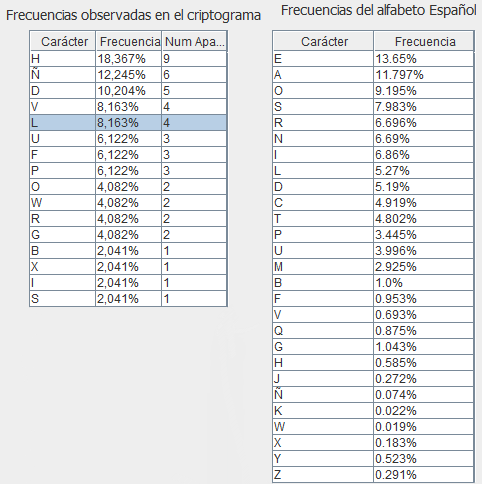
\includegraphics[scale=1]{CC.png} 
% \end{center}

\item \textbf{Con el algoritmo de cifra por multiplicación (Decimación) con $a = 5$, cifre, descifre, y criptoanalice, según estadísticas del lenguaje, el mensaje: \\ M = \emph{El cifrado por multiplicación exige la existencia del inverso en el cuerpo}}. 

Cifrado:

$C_{i}= (a * M_{i}) mod \; 27$

 \begin{multicols}{2} 

$(5*(E)4) \; mod \; 27 = (T)20$ \\
$(5*(L)11 \; mod \; 27 = (B)1$ \\
$(5*(C)2 \; mod \; 27 = (K)10$\\
$(5*(I)8 \; mod \; 27 = (N)13$ \\
$(5*(F)5 \; mod \; 27 = (Y)25$ \\
$(5*(R)18 \; mod \; 27 = (J)9$ \\
$(5*(A)0 \; mod \; 27 = (A)0$ \\
$(5*(D)3 \; mod \; 27 = (O)15$ \\
$(5*(O)15 \; mod \; 27 = (U)21$ \\
$(5*(P)16 \; mod \; 27 = (Z)26$ \\
$(5*(O)15 \; mod \; 27 = (U)21$ \\
$(5*(R)18 \; mod \; 27 = (J)9$ \\
$(5*(M)12 \; mod \; 27 = (G)6$ \\
$(5*(U)21 \; mod \; 27 = (X)24$ \\
$(5*(L)11 \; mod \; 27 = (B)1$ \\
$(5*(T)20 \; mod \; 27 = (S)19$ \\
$(5*(I)8 \; mod \; 27 = (N)13$ \\
$(5*(C)2 \; mod \; 27 = (K)10$\\
$(5*(A)0 \; mod \; 27 = (A)0$ \\
$(5*(C)2 \; mod \; 27 = (K)10$\\
$(5*(I)8 \; mod \; 27 = (N)13$ \\
$(5*(O)15 \; mod \; 27 = (U)21$ \\
$(5*(N)13 \; mod \; 27 = (L)11$ \\
$(5*(E)4) \; mod \; 27 = (T)20$ \\
$(5*(X)24) \; mod \; 27 = (M)12$ \\
$(5*(I)8 \; mod \; 27 = (N)13$ \\
$(5*(G)6 \; mod \; 27 = (D)3$ \\
$(5*(E)4) \; mod \; 27 = (T)20$ \\
$(5*(L)11 \; mod \; 27 = (B)1$ \\
$(5*(A)0 \; mod \; 27 = (A)0$ \\
$(5*(E)4) \; mod \; 27 = (T)20$ \\
$(5*(X)24) \; mod \; 27 = (M)12$ \\
$(5*(I)8 \; mod \; 27 = (N)13$ \\
$(5*(S)19 \; mod \; 27 = ($\textit{Ñ}$)14$ \\
$(5*(T)20 \; mod \; 27 = (S)19$ \\
$(5*(E)4) \; mod \; 27 = (T)20$ \\
$(5*(N)13 \; mod \; 27 = (L)11$ \\
$(5*(C)2 \; mod \; 27 = (K)10$\\
$(5*(I)8 \; mod \; 27 = (N)13$ \\
$(5*(A)0 \; mod \; 27 = (A)0$ \\
$(5*(D)3 \; mod \; 27 = (O)15$ \\
$(5*(E)4) \; mod \; 27 = (T)20$ \\
$(5*(L)11 \; mod \; 27 = (B)1$ \\
$(5*(I)8 \; mod \; 27 = (N)13$ \\
$(5*(N)13 \; mod \; 27 = (L)11$ \\
$(5*(V)22 \; mod \; 27 = (C)2$ \\
$(5*(E)4) \; mod \; 27 = (T)20$ \\
$(5*(R)18 \; mod \; 27 = (J)9$ \\
$(5*(S)19 \; mod \; 27 = ($\textit{Ñ}$)14$ \\
$(5*(O)15 \; mod \; 27 = (U)21$ \\
$(5*(E)4) \; mod \; 27 = (T)20$ \\
$(5*(N)13 \; mod \; 27 = (L)11$ \\
$(5*(E)4) \; mod \; 27 = (T)20$ \\
$(5*(L)11 \; mod \; 27 = (B)1$ \\
$(5*(C)2 \; mod \; 27 = (K)10$\\
$(5*(U)21 \; mod \; 27 = (X)24$ \\
$(5*(E)4) \; mod \; 27 = (T)20$ \\
$(5*(R)18 \; mod \; 27 = (J)9$ \\
$(5*(P)16 \; mod \; 27 = (Z)26$ \\
$(5*(O)15 \; mod \; 27 = (U)21$ \\
 \end{multicols}


C = T B K N Y J A O U Z U J G X B S N Z B N K A K N U L T M N D T B A T M N Ñ S T L K N A O T B N L C T Ñ U T L T B K X T J Z U


Descifra : $M_{i}= (a^{-1}* C_{i}) mod \; 27$ \\

$5^{-1} \; mod \; 27 = 11$

\begin{multicols}{2}

$(11 * (T)20) mod \; 27= (E) 4 $\\
$(11 * (B)1) mod \; 27= (L)11 $\\
$(11 * (K)10) mod \; 27= (C)2 $\\
$(11 * (N)13) mod \; 27= (I)8 $\\
$(11 * (Y)25) mod \; 27= (F)5 $\\
$(11 * (J)9) mod \; 27= (R)18 $\\
$(11 * (A)0) mod \; 27= (A)0 $\\
$(11 * (O)15) mod \; 27= (D)3 $\\
$(11 * (U)21) mod \; 27= (O)15 $\\
$(11 * (Z)26) mod \; 27= (P)16 $\\
$(11 * (U)21) mod \; 27= (O)15 $\\
$(11 * (J)9) mod \; 27= (R)18 $\\
$(11 * (G)6) mod \; 27= (M)12 $\\
$(11 * (X)24) mod \; 27= (U)21 $\\
$(11 * (B)1) mod \; 27= (L)11 $\\
$(11 * (S)19) mod \; 27= (T)20 $\\
$(11 * (N)13) mod \; 27= (I)8 $\\
$(11 * (Z)26) mod \; 27= (P)16 $\\
$(11 * (B)1) mod \; 27= (L)11 $\\
$(11 * (N)13) mod \; 27= (I)8 $\\
$(11 * (K)10) mod \; 27= (C)2 $\\
$(11 * (A)0) mod \; 27= (A)0 $\\
$(11 * (K)10) mod \; 27= (C)2 $\\
$(11 * (N)13) mod \; 27= (I)8 $\\
$(11 * (U)21) mod \; 27= (O)15 $\\
$(11 * (L)11) mod \; 27= (N)13 $\\
$(11 * (T)20) mod \; 27= (E) 4 $\\
$(11 * (M)12) mod \; 27= (X) 24 $\\
$(11 * (N)13) mod \; 27= (I)8 $\\
$(11 * (D)3) mod \; 27= (G)6 $\\
$(11 * (T)20) mod \; 27= (E) 4 $\\
$(11 * (B)1) mod \; 27= (L)11 $\\
$(11 * (A)0) mod \; 27= (A)0 $\\
$(11 * (T)20) mod \; 27= (E) 4 $\\
$(11 * (M)12) mod \; 27= (X) 24 $\\
$(11 * (N)13) mod \; 27= (I)8 $\\
$(11 * (\text{\textit{Ñ}})14) mod \; 27= (S)19 $\\
$(11 * (S)19) mod \; 27= (T)20 $\\
$(11 * (T)20) mod \; 27= (E) 4 $\\
$(11 * (L)11) mod \; 27= (N)13 $\\
$(11 * (K)10) mod \; 27= (C)2 $\\
$(11 * (N)13) mod \; 27= (I)8 $\\
$(11 * (A)0) mod \; 27= (A)0 $\\
$(11 * (O)15) mod \; 27= (D)3 $\\
$(11 * (T)20) mod \; 27= (E) 4 $\\
$(11 * (B)1) mod \; 27= (L)11 $\\
$(11 * (N)13) mod \; 27= (I)8 $\\
$(11 * (L)11) mod \; 27= (N)13 $\\
$(11 * (C)2) mod \; 27= (V)22 $\\
$(11 * (T)20) mod \; 27= (E) 4 $\\
$(11 * (\text{\textit{Ñ}})14) mod \; 27= (S)19 $\\
$(11 * (U)21) mod \; 27= (O)15 $\\
$(11 * (T)20) mod \; 27= (E) 4 $\\
$(11 * (L)11) mod \; 27= (N)13 $\\
$(11 * (T)20) mod \; 27= (E) 4 $\\
$(11 * (B)1) mod \; 27= (L)11 $\\
$(11 * (K)10) mod \; 27= (C)2 $\\
$(11 * (X)24) mod \; 27= (U)21 $\\
$(11 * (T)20) mod \; 27= (E) 4 $\\
$(11 * (J)9) mod \; 27= (R)18 $\\
$(11 * (Z)26) mod \; 27= (P)16 $\\
$(11 * (U)21) mod \; 27= (O)15 $\\

\end{multicols}

\begin{tabular}{|c|c|c|}
\hline 
\multicolumn{3}{|c|}{Frecuencias observadas en el criptograma} \\ \hline
Carácter & Frecuencia & Num Apariciones \\ \hline 
E & 15,873\% & 10  \\ \hline
I & 12,698\% & 8  \\ \hline
L & 9,524\% & 6  \\ \hline
O & 7,937\% & 5  \\ \hline
C & 7,937\% & 5  \\ \hline
N & 6,349\% & 4  \\ \hline
A & 6,349\% & 4 \\ \hline
R & 6,349\% & 4  \\ \hline
P & 4,762\% & 3  \\ \hline
S & 3,175\% & 2  \\ \hline
X & 3,175\% & 2 \\ \hline
T & 3,175\% & 2  \\ \hline
U & 3,175\% & 2 \\ \hline
D & 3,175\% & 2 \\ \hline
V & 1,587\% & 1 \\ \hline
F & 1,587\% & 1 \\  \hline
M & 1,587\% & 1 \\  \hline
G & 1,587\% & 1 \\  \hline

\end{tabular}
%\caption{Frecuencias observadas en el criptograma}
\label{tabla:sencilla}


\begin{tabular}{|c|c|c|c|}
\hline 
\multicolumn{4}{|c|}{Frecuencias del alfabeto Esapñol} \\ \hline
Carácter & Frecuencia & Carácter & Frecuencia\\ \hline
E & 13.65\%   & B & 1.0\% \\ \hline
A & 11.797\% & F & 0.953\% \\ \hline
O & 9.195\%  & V & 0.693\% \\ \hline
S & 7.983\%  & Q & 0.875\% \\ \hline
R & 6.696\%& G & 1.043\% \\ \hline
N & 6.69\% & H & 0.585\% \\ \hline
I & 6.86\% & J & 0.272\% \\ \hline
L & 5.27\% & Ñ & 0.074\% \\ \hline
D & 5.19\% & K & 0.022\% \\ \hline
C & 4.919\% & W & 0.019\% \\ \hline
T & 4.802\% & X & 0.183\% \\ \hline
P & 3.996\% & Y & 0.523\% \\ \hline
U & 3.445\% & Z & 0.291\% \\ \hline
M & 2.925\% &   & \\
\hline
\end{tabular}
%\caption{}%
\label{tabla:sencilla}

\item \textbf{Con el algoritmo de cifra afín (a = 7, b = 10) cifre, descifre y criptoanaliza, según estadísticas del lenguaje, el mensaje: \\ M =\emph{ Si tenemos un texto de unos cuantos caracteres, el ataque al criptograma es muy sencillo.}} 

 Cifrado: 
 
  $C_i=(M_i*a+b) mod \thinspace 27$
 

 \begin{multicols}{2} 
 $(S(19)*7+10)mod \thinspace 27 = I (8)$\\
 $(I(8)*7+10)mod \thinspace 27 = M (12)$\\
 $(T(20)*7+10)mod \thinspace 27 = O (15)$\\
 $(E(4)*7+10)mod \thinspace 27 = L (11)$\\
 $(N(13)*7+10)mod \thinspace 27 = T (20)$\\
 $(E(4)*7+10)mod \thinspace 27 = L (11)$\\
 $(M(12)*7+10)mod \thinspace 27 = N (13)$\\
 $(O(15)*7+10)mod \thinspace 27 = H (7)$\\
 $(S(19)*7+10)mod \thinspace 27 = I (8)$\\
 $(U(21)*7+10)mod \thinspace 27 = V (22)$\\
 $(N(13)*7+10)mod \thinspace 27 = T (20)$\\
 $(T(20)*7+10)mod \thinspace 27 = O (15)$\\
 $(E(4)*7+10)mod \thinspace 27 = L (11)$\\
 $(X(24)*7+10)mod \thinspace 27 = P (16)$\\
 $(T(20)*7+10)mod \thinspace 27 = O (15)$\\
 $(O(15)*7+10)mod \thinspace 27 = H (7)$\\
 $(D(3)*7+10)mod \thinspace 27 = E (4)$\\
 $(E(4)*7+10)mod \thinspace 27 = L (11)$\\
 $(U(21)*7+10)mod \thinspace 27 = V (22)$\\
 $(N(13)*7+10)mod \thinspace 27 = T (20)$\\
 $(O(15)*7+10)mod \thinspace 27 = H (7)$\\
 $(S(19)*7+10)mod \thinspace 27 = I (8)$\\
 $(C(19)*7+10)mod \thinspace 27 = X (24)$\\
 $(U(21)*7+10)mod \thinspace 27 = V (22)$\\
 $(A(0)*7+10)mod \thinspace 27 = K (10)$\\
 $(N(13)*7+10)mod \thinspace 27 = T (20)$\\
 $(T(20)*7+10)mod \thinspace 27 = O (15)$\\
 $(O(15)*7+10)mod \thinspace 27 = H (7)$\\
 $(S(19)*7+10)mod \thinspace 27 = I (8)$\\
 $(C(2)*7+10)mod \thinspace 27 = X (24)$\\
 $(A(0)*7+10)mod \thinspace 27 = K (10)$\\
 $(R(18)*7+10)mod \thinspace 27 = B (1)$\\
 $(A(0)*7+10)mod \thinspace 27 = K (10)$\\
 $(C(2)*7+10)mod \thinspace 27 = X (24)$\\
 $(T(20)*7+10)mod \thinspace 27 = O (15)$\\
 $(E(4)*7+10)mod \thinspace 27 = L (11)$\\
 $(R(18)*7+10)mod \thinspace 27 = B (1)$\\
 $(E(4)*7+10)mod \thinspace 27 = L (11)$\\
 $(S(19)*7+10)mod \thinspace 27 = I (8)$\\
 $(E(4)*7+10)mod \thinspace 27 = L (11)$\\
 $(L(11)*7+10)mod \thinspace 27 = G (6)$\\
 $(A(0)*7+10)mod \thinspace 27 = K (10)$\\
 $(T(20)*7+10)mod \thinspace 27 = O (15)$\\
 $(A(0)*7+10)mod \thinspace 27 = K (10)$\\
 $(Q(17)*7+10)mod \thinspace 27 = U (21)$\\
 $(U(21)*7+10)mod \thinspace 27 = V (22)$\\
 $(E(4)*7+10)mod \thinspace 27 = L (11)$\\
 $(A(0)*7+10)mod \thinspace 27 = K (10)$\\
 $(L(11)*7+10)mod \thinspace 27 = G (6)$\\
 $(C(2)*7+10)mod \thinspace 27 = X (24)$\\
 $(R(18)*7+10)mod \thinspace 27 = B (1)$\\
 $(I(8)*7+10)mod \thinspace 27 = M (12)$\\
 $(P(18)*7+10)mod \thinspace 27 = $ \textit{Ñ} $ (14)$\\
 $(T(20)*7+10)mod \thinspace 27 = O (15)$\\
 $(O(15)*7+10)mod \thinspace 27 = H (7)$\\
 $(G(6)*7+10)mod \thinspace 27 = Y (25)$\\
 $(R(18)*7+10)mod \thinspace 27 = B (1)$\\
 $(A(0)*7+10)mod \thinspace 27 = K (10)$\\
 $(M(12)*7+10)mod \thinspace 27 = N (13)$\\
 $(A(0)*7+10)mod \thinspace 27 = K (10)$\\
 $(E(4)*7+10)mod \thinspace 27 = L (11)$\\
 $(S(19)*7+10)mod \thinspace 27 = I (8)$\\
 $(M(12)*7+10)mod \thinspace 27 = N (13)$\\
 $(U(21)*7+10)mod \thinspace 27 = V (22)$\\
 $(Y(25)*7+10)mod \thinspace 27 = W (23)$\\
 $(S(19)*7+10)mod \thinspace 27 = I (8)$\\
 $(E(4)*7+10)mod \thinspace 27 = L (11)$\\
 $(N(13)*7+10)mod \thinspace 27 = T (20)$\\
 $(C(2)*7+10)mod \thinspace 27 = X (24)$\\
 $(I(8)*7+10)mod \thinspace 27 = M (12)$\\
 $(L(11)*7+10)mod \thinspace 27 = G (6)$\\
 $(L(11)*7+10)mod \thinspace 27 = G (6)$\\
 $(O(15)*7+10)mod \thinspace 27 = H (7)$\\
 
 \end{multicols}
 
 
 C = I M O L T L N H I V T O L P O H E L V T H I X V K T O H I X K B K X O L B L I L G K O K U V L K G X B M Ñ O H Y B K N K L I N V W I L T X M G G H
 
 Fórmula descifrado:  $M_i=(C_i-b)*a^{-1} mod \thinspace 27$

\begin{multicols}{2}
$(I(8)-10)*7^{-1} mod \thinspace 27= E (4) $ \\

\end{multicols}


\begin{tabular}{|l|l|l|}
\hline 
Carácter & Frecuencia & Num Apariciones \\ \hline 
E & 13.699\% & 10 \\ \hline
A & 10,959\% & 8 \\ \hline
T & 9,589\% & 7 \\ \hline
S & 9,589\% & 7 \\ \hline
O & 8,219\% & 6 \\ \hline
C & 6,849\% & 5 \\ \hline
U & 6,849\% & 5 \\ \hline
N & 6,849\% & 5 \\ \hline
L & 5,479\% & 4 \\ \hline
R & 5,479\% & 4 \\ \hline
M & 4,110\% & 3 \\ \hline
I & 4,110\% & 3 \\ \hline
Y & 1,370\% & 1 \\ \hline
X & 1,370\% & 1 \\ \hline
D & 1,370\% & 1 \\ \hline
Q & 1,370\% & 1 \\ \hline
P & 1,370\% & 1 \\ \hline
G & 1,370\% & 1 \\ 
\hline
\end{tabular}
%\caption{}%
\label{tabla:sencilla}



\begin{tabular}{|l|l|l|l|}
\hline 
Carácter & Frecuencia & Carácter & Frecuencia \\ \hline
E & 13.68\% & B & 1.42\% \\ \hline
A & 12.53\% & G & 1.01\% \\ \hline
O & 8.68\% & V & 0.9\% \\ \hline
S & 7.98\% & Q & 0.88\% \\ \hline
R & 6.87\% & F & 0.69\% \\ \hline
N & 6.71\% & Ñ & 0.074\% \\ \hline
I & 6.25\% & J & 0.44\% \\ \hline
D & 5.86\% & H & 0.7\% \\ \hline
C & 5.68\% & W & 0.02\% \\ \hline
L & 4.97\% & K & 0.011\% \\ \hline
T & 4.63\% & X & 0.22\% \\ \hline
U & 3.93\% & Y & 0.9\% \\ \hline
M & 3.15\% & Z & 0.52\% \\ \hline
P & 2.51\%  & &  \\ \hline
\end{tabular}
%\caption{}
\label{tabla:sencilla}


% \begin{center}
%    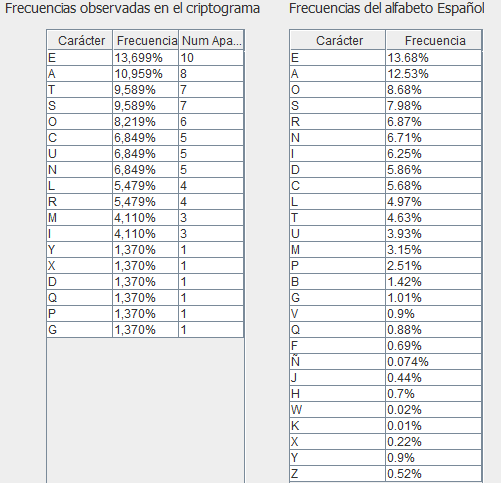
\includegraphics[scale=1]{E3.png} 
% \end{center}
 
 
\item \textbf{Con el algoritmo de Vigènere cuya calve es K = GOL, cifre, descifre, y criptoanalize el mensaje: \\ M = \emph{El jugador se adentró al área y de un golpe preciso introdujo el balón en la portería de aquel desgraciado portero. Era el presagio de lo que iba a ser aquella fatídica tarde para Manolo, justo en el día en que debutaba en aquel estadio.}}  


Cifrado: $C_{i} = M_{i} + K_{i} \;  mod \; 27$


\begin{multicols}{2}
$K (10) = E(4) + G (6) mod \; 27$ \\
$Z (26) = L(11) + O (15) mod \; 27$ \\
$T (20) = J(9) + L (11) mod \; 27$ \\
$A (0) = U(21) + G (6) mod \; 27$ \\
$U (21) = G(6) + O (15) mod \; 27$ \\
$L (11) = A(0) + L (11) mod \; 27$ \\
$J (9) = D(3) + G (6) mod \; 27$ \\
$D (3) = O(15) + O (15) mod \; 27$ \\
$C (2) = R(18) + L (11) mod \; 27$ \\
$Y (25) = S(19) + G (6) mod \; 27$ \\
$S (19) = E(4) + O (15) mod \; 27$ \\
$L (11) = A(0) + L (11) mod \; 27$ \\
$J (9) = D(3) + G (6) mod \; 27$ \\
$S (19) = E(4) + O (15) mod \; 27$ \\
$X (24) = N(13) + L (11) mod \; 27$ \\
$Z (26) = T(20) + G (6) mod \; 27$ \\
$G (6) = R(18) + O (15) mod \; 27$ \\
$Z (26) = O(15) + L (11) mod \; 27$ \\
$G (6) = A(0) + G (6) mod \; 27$ \\
$Z (26) = L(11) + O (15) mod \; 27$ \\
$L (11) = A(0) + L (11) mod \; 27$ \\
$X (24) = R(18) + G (6) mod \; 27$ \\
$S (19) = E(4) + O (15) mod \; 27$ \\
$L (11) = A(0) + L (11) mod \; 27$ \\
$E (4) = Y(25) + G (6) mod \; 27$ \\
$R (18) = D(3) + O (15) mod \; 27$ \\
$O (15) = E(4) + L (11) mod \; 27$ \\
$A (0) = U(21) + G (6) mod \; 27$ \\
$R (18) = D(3) + O (15) mod \; 27$ \\
$O (15) = E(4) + L (11) mod \; 27$ \\
$A (0) = U(21) + G (6) mod \; 27$ \\
$B (1) = N(13) + O (15) mod \; 27$ \\
$Q (17) = G(6) + L (11) mod \; 27$ \\
$U (21) = O(15) + G (6) mod \; 27$ \\
$Z (26) = L(11) + O (15) mod \; 27$ \\
$A (0) = P(16) + L (11) mod \; 27$ \\
$K (10) = E(4) + G (6) mod \; 27$ \\
$E (4) = P(16) + O (15) mod \; 27$ \\
$C (2) = R(18) + L (11) mod \; 27$ \\
$K (10) = E(4) + G (6) mod \; 27$ \\
$Q (17) = C(2) + O (15) mod \; 27$ \\
$S (19) = I(8) + L (11) mod \; 27$ \\
$Y (25) = S(19) + G (6) mod \; 27$ \\
$D (3) = O(15) + O (15) mod \; 27$ \\
$S (19) = I(8) + L (11) mod \; 27$ \\
$S (19) = N(13) + G (6) mod \; 27$ \\
$I (8) = T(20) + O (15) mod \; 27$ \\
$C (2) = R(18) + L (11) mod \; 27$ \\
$U (21) = O(15) + G (6) mod \; 27$ \\
$R (18) = D(3) + O (15) mod \; 27$ \\
$F (5) = U(21) + L (11) mod \; 27$ \\
$O (15) = J(9) + G (6) mod \; 27$ \\
$D (3) = O(15) + O (15) mod \; 27$ \\
$O (15) = E(4) + L (11) mod \; 27$ \\
$Q (17) = L(11) + G (6) mod \; 27$ \\
$P (16) = B(1) + O (15) mod \; 27$ \\
$L (11) = A(0) + L (11) mod \; 27$ \\
$Q (17) = L(11) + G (6) mod \; 27$ \\
$D (3) = O(15) + O (15) mod \; 27$ \\
$X (24) = N(13) + L (11) mod \; 27$ \\
$K (10) = E(4) + G (6) mod \; 27$ \\
$B (1) = N(13) + O (15) mod \; 27$ \\
$V (22) = L(11) + L (11) mod \; 27$ \\
$G (6) = A(0) + G (6) mod \; 27$ \\
$E (4) = P(16) + O (15) mod \; 27$ \\
$Z (26) = O(15) + L (11) mod \; 27$ \\
$X (24) = R(18) + G (6) mod \; 27$ \\
$I (8) = T(20) + O (15) mod \; 27$ \\
$O (15) = E(4) + L (11) mod \; 27$ \\
$X (24) = R(18) + G (6) mod \; 27$ \\
$W (23) = I(8) + O (15) mod \; 27$ \\
$L (11) = A(3) + L (11) mod \; 27$ \\
$J (9) = D(3) + G (6) mod \; 27$ \\
$S (19) = E(4) + O (15) mod \; 27$ \\
$L (11) = A(3) + L (11) mod \; 27$ \\
$W (23) = Q(17) + G (6) mod \; 27$ \\
$J (9) = U(21) + O (15) mod \; 27$ \\
$O (15) = E(4) + L (11) mod \; 27$ \\
$Q (17) = L(11) + G (6) mod \; 27$ \\
$R (18) = D(3) + O (15) mod \; 27$ \\
$O (15) = E(4) + L (11) mod \; 27$ \\
$Y (25) = S(19) + G (6) mod \; 27$ \\
$U (21) = G(6) + O (15) mod \; 27$ \\
$C (2) = R(18) + L (11) mod \; 27$ \\
$G (6) = A(0) + G (6) mod \; 27$ \\
$Q (17) = C(2) + O (15) mod \; 27$ \\
$S (19) = I(8) + L (11) mod \; 27$ \\
$G (6) = A(0) + G (6) mod \; 27$ \\
$R (18) = D(3) + O (15) mod \; 27$ \\
$Z (26) = O(15) + L (11) mod \; 27$ \\
$V (22) = P(16) + G (6) mod \; 27$ \\
$D (3) = O(15) + O (15) mod \; 27$ \\
$C (2) = R(18) + L (11) mod \; 27$ \\
$Z (26) = T(20) + G (6) mod \; 27$ \\
$S (19) = E(4) + O (15) mod \; 27$ \\
$C (2) = R(18) + L (11) mod \; 27$ \\
$U (21) = O(15) + G (6) mod \; 27$ \\
$S (19) = E(4) + O (15) mod \; 27$ \\
$C (2) = R(18) + L (11) mod \; 27$ \\
$G (6) = A(0) + G (6) mod \; 27$ \\
$S (19) = E(4) + O (15) mod \; 27$ \\
$V (22) = L(11) + L (11) mod \; 27$ \\
$V (22) = P(16) + G (6) mod \; 27$ \\
$G (6) = R(18) + O (15) mod \; 27$ \\
$O (15) = E(4) + L (11) mod \; 27$ \\
$Y (25) = S(19) + G (6) mod \; 27$ \\
$O (15) = A(0) + O (15) mod \; 27$ \\
$Q (17) = G(6) + L (11) mod \; 27$ \\
\textit{Ñ}$ (14) = I(8) + G (6) mod \; 27$ \\
$D (3) = O(15) + O (15) mod \; 27$ \\
\textit{Ñ} $Q (14) = D(3) + L (11) mod \; 27$ \\
$K (10) = E(4) + G (6) mod \; 27$ \\
$Z (26) = L(11) + O (15) mod \; 27$ \\
$Z (26) = O(15) + L (11) mod \; 27$ \\
$W (23) = Q(17) + G (6) mod \; 27$ \\
$J (9) = U(21) + O (15) mod \; 27$ \\
$O (15) = E(4) + L (11) mod \; 27$ \\
\textit{Ñ} $W (14) = I(8) + G (6) mod \; 27$ \\
$P (16) = B(1) + O (15) mod \; 27$ \\
$L (11) = A(0) + L (11) mod \; 27$ \\
$G (6) = A(0) + G (6) mod \; 27$ \\
$H (7) = S(19) + O (15) mod \; 27$ \\
$0 (15) = E(4) + L (11) mod \; 27$ \\
$X (24) = R(18) + G (6) mod \; 27$ \\
$O (15) = A(0) + O (15) mod \; 27$ \\
$B (1) = Q(17) + L (11) mod \; 27$ \\
$A (0) = U(21) + G (6) mod \; 27$ \\
$S (19) = E(4) + O (15) mod \; 27$ \\
$V (22) = L(11) + L (11) mod \; 27$ \\
$Q (17) = L(11) + G (6) mod \; 27$ \\
$O (15) = A(0) + O (15) mod \; 27$ \\
$P (16) = F(5) + L (11) mod \; 27$ \\
$G (6) = A(0) + G (6) mod \; 27$ \\
$I (8) = T(20) + O (15) mod \; 27$ \\
$S (19) = I(8) + L (11) mod \; 27$ \\
$J (9) = D(3) + G (6) mod \; 27$ \\
$W (23) = I(8) + O (15) mod \; 27$ \\
$N (13) = C(2) + L (11) mod \; 27$ \\
$G (6) = A(0) + G (6) mod \; 27$ \\
$I (8) = T(20) + O (15) mod \; 27$ \\
$L (11) = A(0) + L (11) mod \; 27$ \\
$X (24) = R(18) + G (6) mod \; 27$ \\
$R (18) = D(3) + O (15) mod \; 27$ \\
$O (15) = E(4) + L (11) mod \; 27$ \\
$V (22) = P(16) + G (6) mod \; 27$ \\
$O (15) = A(0) + O (15) mod \; 27$ \\
$C (2) = R(18) + L (11) mod \; 27$ \\
$G (6) = A(0) + G (6) mod \; 27$ \\
$A (0) = M(12) + O (15) mod \; 27$ \\
$L (11) = A(0) + L (11) mod \; 27$ \\
$S (19) = N(13) + G (6) mod \; 27$ \\
$D (3) = O(15) + O (15) mod \; 27$ \\
$V (22) = L(11) + L (11) mod \; 27$ \\
$U (21) = O(15) + G (6) mod \; 27$ \\
$X (24) = J(9) + O (15) mod \; 27$ \\
$F (5) = U(21) + L (11) mod \; 27$ \\
$Y (25) = S(19) + G (6) mod \; 27$ \\
$I (8) = T(20) + O (15) mod \; 27$ \\
$Z (26) = O(15) + L (11) mod \; 27$ \\
$K (10) = E(4) + G (6) mod \; 27$ \\
$B (1) = N(13) + O (15) mod \; 27$ \\
$O (15) = E(4) + L (11) mod \; 27$ \\
$Q (17) = L(11) + G (6) mod \; 27$ \\
$R (18) = D(3) + O (15) mod \; 27$ \\
$S (19) = I(8) + L (11) mod \; 27$ \\
$G (6) = A(0) + G (6) mod \; 27$ \\
$S (19) = E(4) + O (15) mod \; 27$ \\
$X (24) = N(13) + L (11) mod \; 27$ \\
$W (23) = Q(17) + G (6) mod \; 27$ \\
$J (9) = U(21) + O (15) mod \; 27$ \\
$O (15) = E(4) + L (11) mod \; 27$ \\
$J (9) = D(3) + G (6) mod \; 27$ \\
$S (19) = E(4) + O (15) mod \; 27$ \\
$M (12) = B(1) + L (11) mod \; 27$ \\
$A (0) = U(21) + G (6) mod \; 27$ \\
$I (8) = T(20) + O (15) mod \; 27$ \\
$L (11) = A(0) + L (11) mod \; 27$ \\
$H (7) = B(1) + G (6) mod \; 27$ \\
$O (15) = A(0) + O (15) mod \; 27$ \\
$O (15) = E(4) + L (11) mod \; 27$ \\
$S (19) = N(13) + G (6) mod \; 27$ \\
$O (15) = A(0) + O (15) mod \; 27$ \\
$B (1) = Q(17) + L (11) mod \; 27$ \\
$A (0) = U(21) + G (6) mod \; 27$ \\
$S (19) = E(4) + O (15) mod \; 27$ \\
$V (22) = L(11) + L (11) mod \; 27$ \\
$K (10) = E(4) + G (6) mod \; 27$ \\
$H (7) = S(19) + O (15) mod \; 27$ \\
$E (4) = T(20) + L (11) mod \; 27$ \\
$G (6) = A(0) + G (6) mod \; 27$ \\ 
$R (18) = D(3) + O (15) mod \; 27$ \\
$S (19) = I(8) + L (11) mod \; 27$ \\
$U (21) = O(15) + G (6) mod \; 27$ \\ 
\end{multicols}



    C= K Z T A U L J D C Y S L J S X Z G Z G Z L X S L E R O A B Q U Z A K E C K Q S Y D S S I C U R F O D O Q P L Q D X K B V G E Z X I O X W L J S L W J O Q R O Y U C G Q S G R Z V D C Z S C U S C G S V V G O Y O Q Ñ D Ñ K Z Z W J O Ñ P L G H O X O B A S V Q O P G I S J W N G I L X R O V O C G A L S D V U X F Y I Z K B O Q R S G S X W J O J S M A I L H O O S O B A S V K H E G R S U.


Descifrado:

$ \text{Si} \; (C_{i}- K_{i}) \ge 0 \rightarrow  M_{i} = C_{i} - K_{i} \;  mod \; 27$

$ \text{Si} \; (C_{i}- K_{i}) < 0 \rightarrow  M_{i} = (C_{i} - K_{i} + L ) \;  mod \; 27$ 

\begin{multicols}{2}

$E (4) = K (10) - G (6)\;  mod \; 27$ \\
$L (11) = Z (26) - O (15)\;  mod \; 27$\\
$J (9) = T (20) - L (11)\;  mod \; 27$ \\
$U (21) = (A (0) - G (6) + 27)\;  mod \; 27$\\
$G (6) = U (21) - O (15)\;  mod \; 27$\\
$A (0) = L (11) - L (11)\;  mod \; 27$\\
$D (3) = J (9) - G (6) \;  mod \; 27$\\
$O (15) =  (D(3) - O (15) + 27)\;  mod \; 27$\\
$R (18) = (C(2) - L (11) + 27)\;  mod \; 27$\\
$S (19) = Y (25) - G (6) \;  mod \; 27$\\
$E (4) = S (19) - O (15)\;  mod \; 27$\\
$A (0) = L (11) - L (11)\;  mod \; 27$\\
$D (3) = J (9) - G (6) \;  mod \; 27$\\
$E (4) = S (19) - O (15)\;  mod \; 27$\\
$N (13) = X (24) - L (11)\;  mod \; 27$\\
$T (20) = Z (26) - G (6) \;  mod \; 27$\\
$R (18) = (G (6) - O (15) + 27)\;  mod \; 27$\\
$O (15) = Z (26) - L (11)\;  mod \; 27$\\
$A (0) = G (6) - G (6) \;  mod \; 27$\\
$L (11) = Z (26) - O (15) \;  mod \; 27$\\
$A (0) = L (11) - L (11)\;  mod \; 27$\\
$R (18) = X (24) - G (6) \;  mod \; 27$\\
$E (4) = S (19) - O (15) \;  mod \; 27$\\
$A (0) = L (11) - L (11)\;  mod \; 27$\\
$Y (25) = (E (4) - G (6) + 27) \;  mod \; 27$\\
$D (3) = R (18) - O (15) \;  mod \; 27$\\
$E (4) = O (15) - L (11)\;  mod \; 27$\\
$U (21) = (A (0) - G (6) + 27) \;  mod \; 27$\\
$N (13) = (B (1) - O (15) + 27) \;  mod \; 27$\\
$G (6) = Q (17) - L (11)\;  mod \; 27$\\
$O (15) = U (21) - G (6) \;  mod \; 27$\\
$L (11) = Z (26) - O (15) \;  mod \; 27$\\
$P (16) = (A (0) - L (11) + 27) \;  mod \; 27$\\
$E (4) = K (10) - G (6) \;  mod \; 27$\\
$P (16) = (E (4) - O (15) +27) \;  mod \; 27$\\
$R (18) = (C (2) - L (11) + 27) \;  mod \; 27$\\
$E (4) = K (10) - G (6) \;  mod \; 27$\\
$C (2) = Q (17) - O (15) \;  mod \; 27$\\
$I (8) = S (19) - L (11)  \;  mod \; 27$\\
$S (19) = Y (25) - G (6) \;  mod \; 27$\\
$O (15) = (D (3) - O (15) +27) \;  mod \; 27$\\
$I (8) = S (19) - L (11)  \;  mod \; 27$\\
$N (13) = S (19) - G (6) \;  mod \; 27$\\
$T (20) = (I (8) - O (15) +27) \;  mod \; 27$\\
$R (18) = (C (2) - L (11) +27)  \;  mod \; 27$\\
$O (15) = U (21) - G (6) \;  mod \; 27$\\
$D (3) = R (18) - O (15)  \;  mod \; 27$\\
$U (21) = (F (5) - L (11) +27)  \;  mod \; 27$\\
$J (9) = O (15) - G (6) \;  mod \; 27$\\
$O (15) = (D (3) - O (15) + 27)  \;  mod \; 27$\\
$E (4) = O (15) - L (11) \;  mod \; 27$\\
$L (11) = Q (17) - G (6) \;  mod \; 27$\\
$B (1) = P (16) - O (15)  \;  mod \; 27$\\
$A (0) = L (11) - L (11) \;  mod \; 27$\\
$L (11) = Q (17) - G (6) \;  mod \; 27$\\
$O (15) = (D (3) - O (15) + 27) \;  mod \; 27$\\
$N (13) = X (24) - L (11) \;  mod \; 27$\\
$E (4) = K (10) - G (6) \;  mod \; 27$\\
$N (13) = (B (1) - O (15) + 27) \;  mod \; 27$\\
$L (11) = V (22) - L (11) \;  mod \; 27$\\
$A (0) = G (6) - G (6) \;  mod \; 27$\\
$P (16) = (E (4) - O (15) + 27) \;  mod \; 27$\\
$O (15) = Z (26) - L (11) \;  mod \; 27$\\
$R (18) = X (24) - G (6) \;  mod \; 27$\\
$T (20) = (I (8) - O (15) + 27) \;  mod \; 27$\\
$E (4) = O (15) - L (11) \;  mod \; 27$\\
$R (18) = X (24) - G (6) \;  mod \; 27$\\
$I (8) = W (23) - O (15) \;  mod \; 27$\\
$A (0) = L (11) - L (11) \;  mod \; 27$\\
$D (3) = J (9) - G (6) \;  mod \; 27$\\
$E (4) = S (19) - O (15) \;  mod \; 27$\\
$A (0) = L (11) - L (11) \;  mod \; 27$\\
$Q (17) = W (23) - G (6) \;  mod \; 27$\\
$U (21) = (J (9) - O (15) +27) \;  mod \; 27$\\
$E (4) = O (15) - L (11) \;  mod \; 27$\\
$L (11) = Q (17) - G (6) \;  mod \; 27$\\
$D (3) = R (18) - O (15) \;  mod \; 27$\\
$E (4) = O (15) - L (11) \;  mod \; 27$\\
$S (19) = Y (25) - G (6) \;  mod \; 27$\\
$G (6) = U (21) - O (15) \;  mod \; 27$\\
$R (18) = (C (2) - L (11) +27) \;  mod \; 27$\\
$A (0) = G (6) - G (6) \;  mod \; 27$\\
$C (2) = Q (17) - O (15) \;  mod \; 27$\\
$I (8) = S (19) - L (11) \;  mod \; 27$\\
$A (0) = G (6) - G (6) \;  mod \; 27$\\
$D (3) = R (18) - O (15) \;  mod \; 27$\\
$O (15) = Z (26) - L (11) \;  mod \; 27$\\
$P (16) = V (22) - G (6) \;  mod \; 27$\\
$O (15) = (D (3) - O (15) + 27) \;  mod \; 27$\\
$R (18) = (C (2) - L (11)+ 27) \;  mod \; 27$\\
$T (20) = Z (26) - G (6) \;  mod \; 27$\\
$E (4) = S (19) - O (15) \;  mod \; 27$\\
$R (18) = (C (2) - L (11)+ 27) \;  mod \; 27$\\
$O (15) = U (21) - G (6) \;  mod \; 27$\\
$E (4) = S (19) - O (15) \;  mod \; 27$\\
$R (18) = (C (2) - L (11)+ 27) \;  mod \; 27$\\
$A (0) = G (6) - G (6) \;  mod \; 27$\\
$E (4) = S (19) - O (15) \;  mod \; 27$\\
$L (11) = V (22) - L (11) \;  mod \; 27$\\
$P (16) = V (22) - G (6) \;  mod \; 27$\\
$R (18) = (G (6) - O (15) + 27) \;  mod \; 27$\\
$E (4) = O (15) - L (11) \;  mod \; 27$\\
$S (19) = Y (25) - G (6) \;  mod \; 27$\\
$A (0) = O (15) - O (15) \;  mod \; 27$\\
$G (6) = Q (17) - L (11) \;  mod \; 27$\\
$I (8) = \text{\textit{Ñ}} (14) - G (6) \;  mod \; 27$\\
$O (15) = (D (3) - O (15) + 27) \;  mod \; 27$\\
$D (3) = \text{\textit{Ñ}} (14) - L (11) \;  mod \; 27$\\
$E (4) = K (10) - G (6) \;  mod \; 27$\\
$L (11) = Z (26) - O (15) \;  mod \; 27$\\
$O (15) = Z (26) - L (11) \;  mod \; 27$\\
$Q (17) = W (23) - G (6) \;  mod \; 27$\\
$U (21) = (J (9) - O (15) + 27) \;  mod \; 27$\\
$E (4) = O (15) - L (11) \;  mod \; 27$\\
$I (8) = \text{\textit{Ñ}} (14) - G (6) \;  mod \; 27$\\
$B (1) = P (16) - O (15)  \;  mod \; 27$\\
$A (0) = L (11) - L (11) \;  mod \; 27$\\
$A (0) = G (6) - G (6) \;  mod \; 27$\\
$S (19) = (H (7) - O (15) + 27)  \;  mod \; 27$\\
$E (4) = O (15) - L (11) \;  mod \; 27$\\
$R (18) = X (24) - G (6) \;  mod \; 27$\\
$A (0) = O (15) - O (15) \;  mod \; 27$\\
$Q (17) = (B (1) - L (11) + 27) \;  mod \; 27$\\
$U (21) = (A (0) - G (6) + 27) \;  mod \; 27$\\
$E (4) = S (19) - O (15) \;  mod \; 27$\\
$L (11) = V (22) - L (11) \;  mod \; 27$\\
$L (11) = Q (17) - G (6) \;  mod \; 27$\\
$A (0) = O (15) - O (15) \;  mod \; 27$\\
$F (5) = P (16) - L (11) \;  mod \; 27$\\
$A (0) = G (6) - G (6) \;  mod \; 27$\\
$T (20) = (I (8) - O (15) + 27) \;  mod \; 27$\\
$I (8) = S (19) - L (11) \;  mod \; 27$\\
$D (3) = J (9) - G (6) \;  mod \; 27$\\
$I (8) = W (23) - O (15) \;  mod \; 27$\\
$C (2) = N (13) - L (11) \;  mod \; 27$\\
$A (0) = G (6) - G (6) \;  mod \; 27$\\
$T (20) = (I (8) - O (15) + 27) \;  mod \; 27$\\
$A (0) = L (11) - L (11) \;  mod \; 27$\\
$R (18) = X (24) - G (6) \;  mod \; 27$\\
$D (3) = R (18) - O (15) \;  mod \; 27$\\
$E (4) = O (15) - L (11) \;  mod \; 27$\\
$P (16) = V (22) - G (6) \;  mod \; 27$\\
$A (0) = O (15) - O (15) \;  mod \; 27$\\
$R (18) = (C (2) - L (11) +27)  \;  mod \; 27$\\
$A (0) = G (6) - G (6) \;  mod \; 27$\\
$M (12) = (A (0) - O (15) + 27) \;  mod \; 27$\\
$A (0) = L (2) - L (11)   \;  mod \; 27$\\
$N (12) = S (19) - G (6) \;  mod \; 27$\\
$O (15) = (D (3) - O (15) + 27) \;  mod \; 27$\\
$L (11) = V (22) - L (11)   \;  mod \; 27$\\
$O (15) = U (21) - G (6) \;  mod \; 27 $\\ 
$J (9) = X (24) - O (15) \;  mod \; 27$\\
$U (21) = (F (5) - L (11) + 27)  \;  mod \; 27$\\
$S (19) = Y (25) - G (6) \;  mod \; 27 $\\ 
$T (20) = (I (8) - O (15) + 27) \;  mod \; 27$\\
$O (15) = Z (26) - L (11)  \;  mod \; 27$\\
$E (4) = K (10) - G (6) \;  mod \; 27 $\\ 
$N (13) = (B (1) - O (15) + 27) \;  mod \; 27$\\
$E (4) = O (15) - L (11)  \;  mod \; 27$\\
$L (11) = Q (17) - G (6) \;  mod \; 27 $\\ 
$D (3) = R (18) - O (15)\;  mod \; 27$\\
$I (8) = S (19) - L (11)  \;  mod \; 27$\\
$A (0) = G (6) - G (6) \;  mod \; 27 $\\ 
$E (4) = S (19) - O (15)\;  mod \; 27$\\
$N (13) = X (24) - L (11)  \;  mod \; 27$\\
$Q (17) = W (23) - G (6) \;  mod \; 27 $\\ 
$U (21) = (J (9) - O (15) + 27)\;  mod \; 27$\\
$E (4) = O (15) - L (11)  \;  mod \; 27$\\
$D (3) = J (9) - G (6) \;  mod \; 27 $\\ 
$E (4) = S (19) - O (15) \;  mod \; 27$\\
$B (1) = M (12) - L (11)  \;  mod \; 27$\\
$U (21) = (A (0) - G (6) + 27) \;  mod \; 27 $\\ 
$T (20) = (I (8) - O (15) + 27)\;  mod \; 27$\\
$A (0) = L (11) - L (11)  \;  mod \; 27$\\
$B (1) = H (7) - G (6) \;  mod \; 27 $\\ 
$A (0) = O (15) - O (15)\;  mod \; 27$\\
$E (4) = O (15) - L (11)  \;  mod \; 27$\\
$N (13) = S (19) - G (6) \;  mod \; 27 $\\ 
$A (0) = O (15) - O (15)\;  mod \; 27$\\
$Q (17) = (B (1) - L (11) + 27) \;  mod \; 27$\\
$U (21) = (A (0) - G (6) + 27) \;  mod \; 27 $\\
$E (4) = S (19) - O (15)\;  mod \; 27$\\
$L (11) = V (22) - L (11)  \;  mod \; 27$\\
$E (4) = K (10) - G (6) \;  mod \; 27 $\\
$S (19) = (H (7) - O (15) + 27)\;  mod \; 27$\\
$T (20) = (E (4) - L (11) + 27)  \;  mod \; 27$\\
$A (0) = G (6) - G (6) \;  mod \; 27 $\\
$D (3) = R (18) - O (15) \;  mod \; 27$\\
$I (8) = S (19) - L (11)  \;  mod \; 27$\\
$O (15) = U (21) - G (6) \;  mod \; 27 $\\
\end{multicols}

Criptoanálisis:


\begin{tabular}{|c|c|c|c|c|c|}
\hline 
Palabra & Num & Separación & Palabra & Num & Separación\\ \hline 
PORTER & 2 & 26 & IA & 3 & 16, 78 \\ \hline
AQUEL & 3 & 50.57 & LA & 3 & 40, 67 \\ \hline
NTRO & 2 & 28 & LO & 3 & 55, 40 \\ \hline
QUE & 5 & 39, 11, 43... & OE & 3 & 44, 62 \\ \hline
ADE & 2 & 57 & OR & 3 & 55, 26 \\ \hline
ADO & 2 & 79 & RE & 3 & 14, 65 \\ \hline
AEN & 2 & 13 & RO & 3 & 28, 13 \\ \hline
ELD & 2 & 84 & TA & 3 & 36, 13 \\ \hline
ERA & 2 & 25 & AL & 2 & 35 \\ \hline
IAD &2 & 16 & AT & 2 & 6 \\ \hline
PRE & 2 & 65 & CI & 2 & 45 \\ \hline
EL & 8 & 50, 24, 23... & EP & 2 & 107\\ \hline
DE & 7 & 13, 44, 7... & IO & 2 & 83\\ \hline
AD & 5 &  6, 57, 16... & JU & 2 & 149\\ \hline
EN & 5 &  44, 99, 7, 13... & LP & 2 & 67\\ \hline
ER &  4 &  26, 28, 25... & NE & 2 & 101\\ \hline
RA & 4 & 15, 25, 23 & OD & 2 & 61 \\ \hline
AE & 3 & 66, 13 & OL & 2 & 118\\ \hline
AR & 3 & 117, 5 & SE & 2 & 109\\ \hline
BA & 3 & 63, 59 & ST & 2 & 31\\ \hline
DI & 3 & 28, 27 & & &  \\ \hline
EA & 3 & 28, 27 & & & \\ \hline
ES & 3 & 24, 82 & & & \\ \hline

\end{tabular}
%\caption{}%
\label{tabla:sencilla}


\item \textbf{Cifre y descifre en modo clave continua el mensaje: \\ M = \emph{ Aquí se suma carácter a carácter la cadena de entrada con la clave.} \\ Y la clave siendo: \\K = \emph{ La clave será un texto de longitud igual o mayor que el texto en claro.}}


Cifrado:

$C_i = M_i +K_i \; mod \; 27 $

\begin{multicols}{2}

$L (11) = A (0) + L (11) \; mod \; 27$ \\
$Q (17) = Q (17) + A (0) \; mod \; 27$ \\
$W (23) = U (21) + C (2) \; mod \; 27$ \\
$S (19) = I (8) + L (11) \; mod \; 27$ \\
$S (19) = S (19) + A (0) \; mod \; 27$ \\
$Z (26) = E (4) + V (22) \; mod \; 27$ \\
$W (23) = S (19) + E (4) \; mod \; 27$ \\
$N (13) = U (21) + S (19) \; mod \; 27$ \\
$P (16) = M (12) + E (4) \; mod \; 27$ \\
$R (18) = A (0) + R (18) \; mod \; 27$ \\
$C (2) = C (2) + A (0) \; mod \; 27$ \\
$U (21) = A (0) + U (21) \; mod \; 27$ \\
$E (4) = R (18) + N (13) \; mod \; 27$ \\
$T (20) = A (0) + T (20) \; mod \; 27$ \\
$G (6) = C (2) + E (4) \; mod \; 27$ \\
$Q (17) = T (20) + X (24) \; mod \; 27$ \\
$X (24) = E (4) + T (20) \; mod \; 27$ \\
$G (6) = R (18) + O (15) \; mod \; 27$ \\
$D (3) = A (0) + D (3) \; mod \; 27$ \\
$G (6) = C (2) + E (4) \; mod \; 27$ \\
$L (11) = A (0) + L (11) \; mod \; 27$ \\
$G (6) = R (18) + O (15) \; mod \; 27$ \\
$N (13) = A (0) + N (13) \; mod \; 27$ \\
$I (8) = C (2) + G (6) \; mod \; 27$ \\
$B (1) = T (20) + I (8) \; mod \; 27$ \\
$X (24) = E (4) + T (20) \; mod \; 27$ \\
$M (12) = R (18) + U (21) \; mod \; 27$ \\
$\text{\textit{Ñ}} (14) = L (11) + D (3) \; mod \; 27$ \\
$I (8) = A (0) + I (8) \; mod \; 27$ \\
$I (8) = C (2) + G (6) \; mod \; 27$ \\
$U (21) = A (0) + U (21) \; mod \; 27$ \\
$D (3) = D (3) + A (0) \; mod \; 27$ \\
$O (15) = E (4) + L (11) \; mod \; 27$ \\
$B (1) = N (13) + O (15) \; mod \; 27$ \\
$M (12) = A (0) + M (12) \; mod \; 27$ \\
$D (3) = D (3) + A (0) \; mod \; 27$ \\
$C (2) = E (4) + Y (25) \; mod \; 27$ \\
$S (19) = E (4) + O (15) \; mod \; 27$ \\
$E (4) = N (13) + R (18) \; mod \; 27$ \\
$K (10) = T (20) + Q (17) \; mod \; 27$ \\
$M (12) = R (18) + U (21) \; mod \; 27$ \\
$E (4) = A (0) + E (4) \; mod \; 27$ \\
$H (7) = D (3) + E (4) \; mod \; 27$ \\
$L (11) = A (0) + L (11) \; mod \; 27$ \\
$V (22) = C (2) + T (20) \; mod \; 27$ \\
$S (19) = O (15) + E (4) \; mod \; 27$ \\
$K (10) = N (13) + X (24) \; mod \; 27$ \\
$E (4) = L (11) + T (20) \; mod \; 27$ \\
$O (15) = A (0) + O (15) \; mod \; 27$ \\
$G (6) = C (2) + E (4) \; mod \; 27$ \\
$X (24) = L (11) + N (13) \; mod \; 27$ \\
$C (2) = A (0) + C (2) \; mod \; 27$ \\
$G (6) = V (22) + L (11) \; mod \; 27$ \\
$E (4) = E (4) + A (0) \; mod \; 27$ \\
\end{multicols}


C = L Q W S S Z W N P R C U E T G Q X G D G L G N I B X M Ñ I I U D O B M D C S E K M E H L V S K E O G X C G E


Descifrado:

$ \text{Si} \; (C_{i}- K_{i}) \ge 0 \rightarrow  M_{i} = C_{i} - K_{i} \;  mod \; 27$

$ \text{Si} \; (C_{i}- K_{i}) < 0 \rightarrow  M_{i} = (C_{i} - K_{i} + L ) \;  mod \; 27$ 


\begin{multicols}{2}
$A (0) = L (11) - L (11)\;  mod \; 27$\\
$Q (17) = Q (17) - A (0)\;  mod \; 27$\\
$U (21) = W (23) - C (2)\;  mod \; 27$\\
$I (8) = S (19) - L (11)\;  mod \; 27$\\
$S (11) = S (11) - A (0)\;  mod \; 27$\\
$E (4) = Z (26) - V (22)\;  mod \; 27$\\
$S (19) = W (23) - E (4)\;  mod \; 27$\\
$U (21) = (N (13) - S (19) + 27)\;  mod \; 27$\\
$M (12) = P (16) - E (4)\;  mod \; 27$\\
$A (0) = R (18) - R (18)\;  mod \; 27$\\
$C (2) = C (2) - A (0)\;  mod \; 27$\\
$A (0) = U (21) - U (21)\;  mod \; 27$\\
$R (18) = (E (4) - N (13) + 27)\;  mod \; 27$\\
$A (0) = T (20) - T (20)\;  mod \; 27$\\
$C (2) = G (6) - E (4)\;  mod \; 27$\\
$T (20) = (Q (17) - X (24) + 27)\;  mod \; 27$\\
$E (4) = X (24) - T (20)\;  mod \; 27$\\
$R (18) = (G (6) - O (15) + 27)\;  mod \; 27$\\
$A (0) = D (3) - D (3)\;  mod \; 27$\\
$C (2) = G(6) - E (4)\;  mod \; 27$\\
$A (0) = L (11) - L (11)\;  mod \; 27$\\
$R (18) = (G (6) - O (15) + 27)\;  mod \; 27$\\
$A (0) = N (13) - N (13)\;  mod \; 27$\\
$C (2) = I (8) - G (6)\;  mod \; 27$\\
$T (20) = (B (1) - I (8) + 27)\;  mod \; 27$\\
$E (4) = X (24) - T (20)\;  mod \; 27$\\
$R (18) = (M (12) - U (21) + 27)\;  mod \; 27$\\
$L (11) = \text{\textit{Ñ}} (14) - D (3)\;  mod \; 27$\\
$A (0) = I (8) - I (8)\;  mod \; 27$\\
$C (2) = I (8) - G (6)\;  mod \; 27$\\
$A (0) = U (21) - U (21)\;  mod \; 27$\\
$D (3) = D (3) - A (0)\;  mod \; 27$\\
$E (4) = O (15) - L (11)\;  mod \; 27$\\
$N (13) = (B (1) - O (15) + 27)\;  mod \; 27$\\
$A (0) = M (12) - M (12)\;  mod \; 27$\\
$D (3) = D (3) - A (0)\;  mod \; 27$\\
$E (4) = (C (2) - Y (25) + 27)\;  mod \; 27$\\
$E (4) = S (19) - O (15)\;  mod \; 27$\\
$N (13) = (E (4) - R (18) + 27)\;  mod \; 27$\\
$T (20) = (K (10) - Q (17) + 27)\;  mod \; 27$\\
$R (18) = (M (12) - U (21) + 27)\;  mod \; 27$\\
$A (0) = E (4) - E (4)\;  mod \; 27$\\
$D (3) = H (7) - E (4)\;  mod \; 27$\\
$A (0) = L (11) - L (11)\;  mod \; 27$\\
$C (2) = V (22) - T (20)\;  mod \; 27$\\
$O (15) = S (19) - E (4)\;  mod \; 27$\\
$N (13) = (K (10) - X (24) + 27)\;  mod \; 27$\\
$L (11) = (E (4) - T (20) + 27)\;  mod \; 27$\\
$A (0) = O (15) - O (15)\;  mod \; 27$\\
$C (2) = G (6) - E (4)\;  mod \; 27$\\
$L (11) = X (24) - N (13)\;  mod \; 27$\\
$A (0) = C (2) - C (2)\;  mod \; 27$\\
$V (22) = (G (6) - L (11) + 27)\;  mod \; 27$\\
$E (4) = E (4) - A (0)\;  mod \; 27$\\
\end{multicols}


\item \textbf{Cifre con Vernam binario el mensaje M de 18 caracteres con la clave K de 26 caracteres. . Compruebe la cifra de los tres primeros caracteres. \\
K =\emph{CIFRADOR BINARIO DE VERNAM} \\
M =  \emph{UNA CIFRA POR BITS}}

Cifrado:
\begin{multicols}{2}
$ U \oplus C = 00111 \oplus 01110 = 01001 (D)$ \\
$ N \oplus I = 01100 \oplus 00110 = 01010 (R)$ \\
$ A \oplus F = 00011 \oplus 01101 = 01110 (C)$ \\
$ C \oplus R = 01110 \oplus 01010 = 00100 (5)$ \\
$ I \oplus A = 00110 \oplus 00011 = 00101 (S)$ \\
$ F \oplus D = 01101 \oplus 01001 = 00100 (5)$ \\
$ R \oplus O = 01010 \oplus 11000 = 10010 (L)$ \\
$ A \oplus R = 00011 \oplus 01010 = 01001 (D)$ \\
$ P \oplus B = 10110 \oplus 11001 = 01111 (K)$ \\
$ O \oplus I = 11000 \oplus 00110 = 11110 (V)$ \\
$ R \oplus N= 01010 \oplus 01100 = 00110 (I)$ \\
$ B \oplus A= 11001 \oplus 00011 = 11010 (G)$ \\
$ I \oplus R= 00110 \oplus 01010 = 01100 (N)$ \\
$ T \oplus I= 10000 \oplus 00110 = 10110 (P)$ \\
$ S \oplus O= 00101 \oplus 11000 = 11101 (X)$ \\
\end{multicols}

C=  D R C 5 S 5 L D K V I G N P X


\item \textbf{Cifre i descifre con Hill digrámico mod 27 el mensaje:\\
M = \emph{UN CIFRADOR DE HILL},  con la clave:}
\begin{equation*}
    C= \left(
    \begin{array}{cc}
    7 & 4 \\
    13 & 17
    \end{array}
    \right)
\end{equation*}
Cifrador:
\begin{equation*}
    \left(
    \begin{array}{cc}
    7 & 4 \\
    13 & 17
    \end{array}
    \right) * \left(\begin{array}{c}
    21 \\
    13
    \end{array}
    \right)=\left(\begin{array}{c}
    199 \\
    494
    \end{array}
    \right) = \left(\begin{array}{c}
    10 \\
    8
    \end{array}
    \right) mod \; (27) \Rightarrow \left(\begin{array}{c}
    K \\
    I
    \end{array}
    \right)
\end{equation*}
\begin{equation*}
    \left(
    \begin{array}{cc}
    7 & 4 \\
    13 & 17
    \end{array}
    \right) * \left(\begin{array}{c}
    2 \\
    8
    \end{array}
    \right)=\left(\begin{array}{c}
    46 \\
    162
    \end{array}
    \right) = \left(\begin{array}{c}
    19 \\
    0
    \end{array}
    \right) mod\; (27) \Rightarrow \left(\begin{array}{c}
    S \\
    A
    \end{array}
    \right)
\end{equation*}
\begin{equation*}
    \left(
    \begin{array}{cc}
    7 & 4 \\
    13 & 17
    \end{array}
    \right) * \left(\begin{array}{c}
    5 \\
    18
    \end{array}
    \right)=\left(\begin{array}{c}
    107 \\
    371
    \end{array}
    \right) = \left(\begin{array}{c}
    26 \\
    20
    \end{array}
    \right) mod \; (27)\Rightarrow \left(\begin{array}{c}
    Z \\
    T
    \end{array}
    \right)
\end{equation*}
\begin{equation*}
    \left(
    \begin{array}{cc}
    7 & 4 \\
    13 & 17
    \end{array}
    \right) * \left(\begin{array}{c}
    0 \\
    3
    \end{array}
    \right)=\left(\begin{array}{c}
    12 \\
    51
    \end{array}
    \right) = \left(\begin{array}{c}
    12 \\
    24
    \end{array}
    \right) mod \; (27) \Rightarrow \left(\begin{array}{c}
    M \\
    X
    \end{array}
    \right)
\end{equation*}
\begin{equation*}
    \left(
    \begin{array}{cc}
    7 & 4 \\
    13 & 17
    \end{array}
    \right) * \left(\begin{array}{c}
    15 \\
    18
    \end{array}
    \right)=\left(\begin{array}{c}
    177 \\
    501
    \end{array}
    \right) = \left(\begin{array}{c}
    15 \\
    15
    \end{array}
    \right) mod \; (27) \Rightarrow \left(\begin{array}{c}
    O \\
    O
    \end{array}
    \right)
\end{equation*}
\begin{equation*}
    \left(
    \begin{array}{cc}
    7 & 4 \\
    13 & 17
    \end{array}
    \right) * \left(\begin{array}{c}
    3 \\
    4
    \end{array}
    \right)=\left(\begin{array}{c}
    37 \\
    107
    \end{array}
    \right) = \left(\begin{array}{c}
    10 \\
    26
    \end{array}
    \right) mod \; (27) \Rightarrow \left(\begin{array}{c}
    K \\
    Z
    \end{array}
    \right)
\end{equation*}
\begin{equation*}
    \left(
    \begin{array}{cc}
    7 & 4 \\
    13 & 17
    \end{array}
    \right) * \left(\begin{array}{c}
    7 \\
    8
    \end{array}
    \right)=\left(\begin{array}{c}
    81 \\
    227
    \end{array}
    \right) = \left(\begin{array}{c}
    0 \\
    11
    \end{array}
    \right) mod \; (27) \Rightarrow \left(\begin{array}{c}
    A \\
    L
    \end{array}
    \right)
\end{equation*}
\begin{equation*}
    \left(
    \begin{array}{cc}
    7 & 4 \\
    13 & 17
    \end{array}
    \right) * \left(\begin{array}{c}
    11 \\
    11
    \end{array}
    \right)=\left(\begin{array}{c}
    121 \\
    330
    \end{array}
    \right) = \left(\begin{array}{c}
    13 \\
    6
    \end{array}
    \right) mod \; (27) \Rightarrow \left(\begin{array}{c}
    N \\
    G
    \end{array}
    \right)
\end{equation*}

C= K I S A Z T M X O O K Z A L N G

Descifrado:
\begin{equation*}
    \left(  M \right) = \left( K^{-1} \right) * \left( C \right) mod \; n
\end{equation*}
\begin{equation*}
    \left(
    \begin{array}{cc}
    7 & 4 \\
    13 & 17
    \end{array}
    \right)^{(-1)}  = \left(
    \begin{array}{cc}
    17/67 & -4/67 \\
    -13/67 & 7/67
    \end{array}
    \right)mod \; (27) = \left(
    \begin{array}{cc}
    20 & 8 \\
    26 & 13
    \end{array}
    \right) 
\end{equation*} % MATRIZ INVERSA DE K

\begin{equation*}
    \left(
    \begin{array}{cc}
    20 & 8 \\
    26 & 13
    \end{array}
    \right) *
    \left(
    \begin{array}{c}
    10\\
    8
    \end{array}
    \right) mod \;(27) = \left(
    \begin{array}{c}
    264\\
    364
    \end{array}
    \right) = \left(
    \begin{array}{c}
    21 \\
    13
    \end{array}
    \right) mod \;(27) \Rightarrow \left(
    \begin{array}{c}
    U\\
    N
    \end{array}
    \right)
\end{equation*}
\begin{equation*}
    \left(
    \begin{array}{cc}
    20 & 8 \\
    26 & 13
    \end{array}
    \right) *
    \left(
    \begin{array}{c}
    19\\
    0
    \end{array}
    \right) mod \;(27) = \left(
    \begin{array}{c}
    380\\
    494
    \end{array}
    \right) = \left(
    \begin{array}{c}
    2 \\
    8
    \end{array}
    \right) mod \; (27) \Rightarrow \left(
    \begin{array}{c}
    C\\
    I
    \end{array}
    \right)
\end{equation*}
\begin{equation*}
    \left(
    \begin{array}{cc}
    20 & 8 \\
    26 & 13
    \end{array}
    \right) *
    \left(
    \begin{array}{c}
    26\\
    20
    \end{array}
    \right) mod \;(27) = \left(
    \begin{array}{c}
    680\\
    936
    \end{array}
    \right) = \left(
    \begin{array}{c}
    5 \\
    18
    \end{array}
    \right) mod \; (27) \Rightarrow \left(
    \begin{array}{c}
    F\\
    R
    \end{array}
    \right)
\end{equation*}
\begin{equation*}
    \left(
    \begin{array}{cc}
    20 & 8 \\
    26 & 13
    \end{array}
    \right) *
    \left(
    \begin{array}{c}
    12\\
    24
    \end{array}
    \right) mod \;(27) = \left(
    \begin{array}{c}
    432\\
    624
    \end{array}
    \right) = \left(
    \begin{array}{c}
    0 \\
    3
    \end{array}
    \right) mod \; (27) \Rightarrow \left(
    \begin{array}{c}
    A\\
    D
    \end{array}
    \right)
\end{equation*}
\begin{equation*}
    \left(
    \begin{array}{cc}
    20 & 8 \\
    26 & 13
    \end{array}
    \right) *
    \left(
    \begin{array}{c}
    15\\
    15
    \end{array}
    \right) mod \;(27) = \left(
    \begin{array}{c}
    420\\
    585
    \end{array}
    \right) = \left(
    \begin{array}{c}
    15 \\
    18
    \end{array}
    \right) mod \; (27) \Rightarrow \left(
    \begin{array}{c}
    O\\
    R
    \end{array}
    \right)
\end{equation*}
\begin{equation*}
    \left(
    \begin{array}{cc}
    20 & 8 \\
    26 & 13
    \end{array}
    \right) *
    \left(
    \begin{array}{c}
    10\\
    26
    \end{array}
    \right) mod \;(27) = \left(
    \begin{array}{c}
    408\\
    598
    \end{array}
    \right) = \left(
    \begin{array}{c}
    3 \\
    4
    \end{array}
    \right) mod \; (27) \Rightarrow \left(
    \begin{array}{c}
    D\\
    E
    \end{array}
    \right)
\end{equation*}
\begin{equation*}
    \left(
    \begin{array}{cc}
    20 & 8 \\
    26 & 13
    \end{array}
    \right) *
    \left(
    \begin{array}{c}
    0\\
    11
    \end{array}
    \right) mod \; (27) = \left(
    \begin{array}{c}
    88\\
    143
    \end{array}
    \right) = \left(
    \begin{array}{c}
    7 \\
    8
    \end{array}
    \right) mod \; (27) \Rightarrow \left(
    \begin{array}{c}
    H\\
    I
    \end{array}
    \right)
\end{equation*}
\begin{equation*}
    \left(
    \begin{array}{cc}
    20 & 8 \\
    26 & 13
    \end{array}
    \right) *
    \left(
    \begin{array}{c}
    13\\
    6
    \end{array}
    \right) mod \;(27) = \left(
    \begin{array}{c}
    308\\
    416
    \end{array}
    \right) = \left(
    \begin{array}{c}
    11 \\
    11
    \end{array}
    \right) mod \; (27) \Rightarrow \left(
    \begin{array}{c}
    L\\
    L
    \end{array}
    \right)
\end{equation*}
\end{enumerate}
\newpage
\subsection{Software Hill:}

\begin{enumerate}

\item \textbf{Calcule el determinante y la inversa para comprobar si las siguientes matrices dirgámicas son válidas para cifrar en el cuerpo 27.}

\begin{equation*}
    A) \rightarrow \left(
    \begin{array}{cc}
    7 & 10 \\
    12 & 19
    \end{array}
    \right) \quad B) \rightarrow \left(
    \begin{array}{cc}
    8 & 5 \\
    2 & 8
    \end{array}
    \right)\quad  C) \rightarrow \left(
    \begin{array}{cc}
    18 & 15 \\
    7 & 8
    \end{array}
    \right) 
\end{equation*}


Determinante de A:
\begin{equation*}
    \begin{vmatrix}
    7 & 10 \\
    12 & 19
    \end{vmatrix} \rightarrow Det=
    7*19 - 10*12 = 13
\end{equation*}
Matriz inversa de A:

\begin{equation*}\left(
    \begin{array}{cc}
    7 & 10 \\
    12 & 19
    \end{array} \bigg\vert  \begin{array}{cc}
    1 & 0 \\
    0 & 1
    \end{array}  \right)
     \rightarrow  19*F1-10*F2 \vert 7*F2-12*F1
     \left(
    \begin{array}{cc}
    1 & 0 \\
    0 & 1
    \end{array}\bigg\vert  \begin{array}{cc}
    19/13 & -10/13 \\
    -12/13 & 7/13
    \end{array}
    \right) 
\end{equation*}



\begin{equation*}
    \left(
    \begin{array}{cc}
    19/13 & -10/13 \\
    -12/13 & 7/13
    \end{array}
    \right) = A^{-1}
\end{equation*}
    


 Determinante de B:\begin{equation*}
    \begin{vmatrix}
    8 & 5 \\
    2 & 8
    \end{vmatrix}   \rightarrow Det=
    8*8 - 5*2 = 54 
\end{equation*}
Matriz inversa de B:
\begin{equation*}
\begin{split} 
    & \left(
    \begin{array}{cc}
    8 & 5 \\
    2 & 8
    \end{array} \bigg\vert  \begin{array}{cc}
    1 & 0 \\
    0 & 1
    \end{array}  \right)
     \rightarrow  8*F1-5*F2 \vert 8*F2-2*F1
     \left(
    \begin{array}{cc}
    54 & 0 \\
    0 & 54
    \end{array}\bigg\vert  \begin{array}{cc}
    8 & -5 \\
    -2 & 8
    \end{array}
    \right) \\
    & \rightarrow  F1/54 \vert F2/54 
    \left( \begin{array}{cc}
    1 & 0 \\
    0 & 1
    \end{array}\bigg\vert  \begin{array}{cc}
    4/27 & -5/54 \\
    -1/27 & 4/27
    \end{array}
    \right)
\end{split}
\end{equation*}

\begin{equation*}
    \left( \begin{array}{cc}
    4/27 & -5/54 \\
    -1/27 & 4/27
    \end{array}
    \right)= B^{-1}
\end{equation*}
    


Determinante de C:
 \begin{equation*}
    \begin{vmatrix}
    18 & 15 \\
    7 & 8
    \end{vmatrix} \rightarrow Det=
    18*8 - 15*7 = 39
\end{equation*}
Matriz inversa de C:
\begin{equation*}
    \begin{split}
    C^{-1} &= \frac{(Adj(C)^{T})}{\mid C \mid}\\
    C^{-1} &= \frac{1}{804} \left(
    \begin{array}{cc}
    8 & -15 \\
    -7 & 18
    \end{array}
    \right)\\
    C^{-1} &=  \left(
    \begin{array}{cc}
    8/39 & -5/13 \\
    -7/39 & 6/13
    \end{array}
    \right)
    \end{split}
\end{equation*}

\item \textbf{Calcule el determinante y la inversa para comprobar si las siguientes matrices trigrámicas son válidas para cifrar en el cuerpo 27}



\begin{equation*}
   A = \left(
    \begin{array}{ccc}
    4 & 12 & 9 \\
    5 & 0 & 13 \\
    6 & 8 & 3
    \end{array}
    \right) \quad  B=\left(
    \begin{array}{ccc}
    3 & 12 & 9 \\
    5 & 0 & 13 \\
    6 & 8 & 3
    \end{array}
    \right)
\end{equation*}

Determinante de A:
\begin{equation*}
   \begin{vmatrix}
    4 & 12 & 9 \\
    5 & 0 & 13 \\
    6 & 8 & 3
   \end{vmatrix}    \rightarrow Det=
    4*0*3+12*13*6+9*5*8-9*0*6-4*13*8-12*5*3= 700
\end{equation*}
Matriz inversa de A:
\begin{equation*}
\begin{split}
    A^{-1} &= \frac{(Adj(A)^{T})}{\mid A \mid}\\
    A^{-1} &= \frac{1}{700} \left(
    \begin{array}{ccc}
    -104 & 36 & 156 \\
    63 & -42 & -7 \\
    40 & 40 & -60
    \end{array}
    \right)\\
    A^{-1} &=  \left(
    \begin{array}{ccc}
    -26/175 & 9/175 & 39/175 \\
    9/100 & -3/50 & 1/100 \\
    2/35 & 2/35 & -3/35
    \end{array}
    \right)\\
\end{split}
\end{equation*}

Determinante de B:
\begin{equation*}
    \begin{vmatrix}
    3 & 12 & 9 \\
    5 & 0 & 13 \\
    6 & 8 & 3 
    \end{vmatrix}    \rightarrow Det=
    3*0*3+12*13*6+9*5*8-9*0*6-3*13*8-12*5*3= 804
\end{equation*}
Matriz inversa de B:
\begin{equation*}
\begin{split}
    B^{-1} &= \frac{(Adj(B)^{T})}{\mid B \mid}\\
    B^{-1} &= \frac{1}{804} \left(
    \begin{array}{ccc}
    -104 & 36 & 156 \\
    63 & -45 & 6 \\
    40 & 48 & -60
    \end{array}
    \right)\\
    B^{-1} &=  \left(
    \begin{array}{ccc}
    -26/201 & 3/67 & 13/67 \\
    21/268 & -15/268 & 1/134 \\
    10/201 & 4/67 & -5/67
    \end{array}
    \right)\\
\end{split}
\end{equation*}

\item \textbf{Calcule la inversa de la siguiente matriz pentagrámica en modulo 27:}

\begin{equation*}
\left(
    \begin{array}{ccccc}
    3 & 2 & 1 & 0 & 2  \\
    5 & 5 & 3 & 7 & 1  \\
    8 & 7 & 6 & 5 & 5  \\
    4 & 9 & 6 & 8 & 3  \\
    3 & 9 & 8 & 7 & 3 
   \end{array} \right)
\end{equation*}


\begin{equation*}
    \begin{split}
     &  \left(
    \begin{array}{ccccc|ccccc}
    3 & 2 & 1 & 0 & 2 & 1 & 0 & 0 & 0 & 0 \\
    5 & 5 & 3 & 7 & 1 & 0 & 1 & 0 & 0 & 0 \\
    8 & 7 & 6 & 5 & 5 & 0 & 0 & 1 & 0 & 0 \\
    4 & 9 & 6 & 8 & 3 & 0 & 0 & 0 & 1 & 0 \\
    3 & 9 & 8 & 7 & 3 & 0 & 0 & 0 & 0 & 1
    \end{array}
    \right) \rightarrow\\ 
    & \text{F}1/3 \\ 
    &  \left(
    \begin{array}{ccccc|ccccc}
    1 & 2/3 & 1/3 & 0 & 2/3 & 1/3 & 0 & 0 & 0 & 0 \\
    5 & 5 & 3 & 7 & 1 & 0 & 1 & 0 & 0 & 0 \\
    8 & 7 & 6 & 5 & 5 & 0 & 0 & 1 & 0 & 0 \\
    4 & 9 & 6 & 8 & 3 & 0 & 0 & 0 & 1 & 0 \\
    3 & 9 & 8 & 7 & 3 & 0 & 0 & 0 & 0 & 1
    \end{array}
    \right) \rightarrow  \\
    & F2-5*F1 \vert \text{F}3-\text{F}1*8 \vert \text{F}4-\text{F}1*4 \vert \text{F}5-\text{F}1*3\\
    &  \left(
    \begin{array}{ccccc|ccccc}
    1 & 2/3 & 1/3 & 0 & 2/3 & 1/3 & 0 & 0 & 0 & 0 \\
    0 & 5/3 & 4/3 & 7 & -7/3 & -5/3 & 1 & 0 & 0 & 0 \\
    0 & 5/3 & 0/3 & 5 & -1/3 & -8/3 & 0 & 1 & 0 & 0 \\
    0 & 19/3 & 14/3 & 8 & 1/3 & 4/3 & 0 & 0 & 1 & 0 \\
    0 & 7 & 7 & 7 & 1 & -1 & 0 & 0 & 0 & 1
    \end{array}
    \right) \rightarrow   \\
    & \text{F}2/\frac{5}{3} \\
     &  \left(
    \begin{array}{ccccc|ccccc}
    1 & 2/3 & 1/3 & 0 & 2/3 & 1/3 & 0 & 0 & 0 & 0 \\
    0 & 1 & 4/3 & 21/5 & -7/5 & -1 & 3/5 & 0 & 0 & 0 \\
    0 & 5/3 & 0/3 & 5 & -1/3 & -8/3 & 0 & 1 & 0 & 0 \\
    0 & 19/3 & 14/3 & 8 & 1/3 & 4/3 & 0 & 0 & 1 & 0 \\
    0 & 7 & 7 & 7 & 1 & -1 & 0 & 0 & 0 & 1
    \end{array}  \right) \rightarrow  \\
    & F1-F2*(2/3) \vert \text{F}3-\text{F}2*\frac{5}{3} \vert \text{F}4-\text{F}2*\frac{19}{3} \vert \text{F}5-\text{F}2*7\\
     &  \left(
    \begin{array}{ccccc|ccccc}
    1 & 0 & -1/5 & -14/5 & 8/5 & 1 & -2/5 & 0 & 0 & 0 \\
    0 & 1 & 4/3 & 21/5 & -7/5 & -1 & 3/5 & 0 & 0 & 0 \\
    0 & 0 & 2 & -2 & 2 & -1 & -1 & 1 & 0 & 0 \\
    0 & 0 & -2/5 & -93/5 & 46/5 & 5 & -19/5 & 0 & 1 & 0 \\
    0 & 0 & 7/5 & -112/5 & 54/5 & 6 & -21/5 & 0 & 0 & 1
    \end{array}  \right) \rightarrow  \\ 
    & \text{F}3/2 \\
    &  \left(
    \begin{array}{ccccc|ccccc}
    1 & 0 & -1/5 & -14/5 & 8/5 & 1 & -2/5 & 0 & 0 & 0 \\
    0 & 1 & 4/3 & 21/5 & -7/5 & -1 & 3/5 & 0 & 0 & 0 \\
    0 & 0 & 1 & -1 & 1 & -1/2 & -1/2 & 1/2 & 0 & 0 \\
    0 & 0 & -2/5 & -93/5 & 46/5 & 5 & -19/5 & 0 & 1 & 0 \\
    0 & 0 & 7/5 & -112/5 & 54/5 & 6 & -21/5 & 0 & 0 & 1
    \end{array}  \right) \rightarrow  \\
    & F1-F3*(1/5) \\
     &  \left(
    \begin{array}{ccccc|ccccc}
    1 & 0 & -1/5 & -14/5 & 8/5 & 1 & -2/5 & 0 & 0 & 0 \\
    0 & 1 & 4/3 & 21/5 & -7/5 & -1 & 3/5 & 0 & 0 & 0 \\
    0 & 0 & 1 & -1 & 1 & -1/2 & -1/2 & 1/2 & 0 & 0 \\
    0 & 0 & -2/5 & -93/5 & 46/5 & 5 & -19/5 & 0 & 1 & 0 \\
    0 & 0 & 7/5 & -112/5 & 54/5 & 6 & -21/5 & 0 & 0 & 1
    \end{array}  \right) \rightarrow  \\
    & F1-F3*(1/5) \vert F2-F3*(4/5) \vert F4-F3*(-2/5) \vert F5-F3*(7/5)
\end{split}
\end{equation*}

\begin{equation*}
    \begin{split}
    &  \left(
    \begin{array}{ccccc|ccccc}
    1 & 0 & 0 & -3 & 9/5 & 9/10 & -1/2 & 1/10 & 0 & 0 \\
    0 & 1 & 0 & 5 & -11/5 & -3/5 & 1 & -2/5 & 0 & 0 \\
    0 & 0 & 1 & -1 & 1 & -1/2 & -1/2 & 1/2 & 0 & 0 \\
    0 & 0 & 0 & -19 & 48/5 & 24/5 & -4 & 1/5 & 1 & 0 \\
    0 & 0 & 0 & -21 & 47/5 & 67/10 & -7/2 & -7/10 & 0 & 1
    \end{array}  \right) \rightarrow  \\
    & \text{F}4-19 \\
     &  \left(
    \begin{array}{ccccc|ccccc}
    1 & 0 & 0 & -3 & 9/5 & 9/10 & -1/2 & 1/10 & 0 & 0 \\
    0 & 1 & 0 & 5 & -11/5 & -3/5 & 1 & -2/5 & 0 & 0 \\
    0 & 0 & 1 & -1 & 1 & -1/2 & -1/2 & 1/2 & 0 & 0 \\
    0 & 0 & 0 & 1 & -48/95 & -24/95 & 4/19 & -1/95 & -1/19 & 0 \\
    0 & 0 & 0 & -21 & 47/5 & 67/10 & -7/2 & -7/10 & 0 & 1
    \end{array}  \right) \rightarrow \\
    & \text{F}1-\text{F}4*(-3) \vert \text{F}2-\text{F}4*5 \vert \text{F}3-\text{F}4*(-1) \vert \text{F}5-\text{F}4*(-21)\\
    &  \left(
    \begin{array}{ccccc|ccccc}
    1 & 0 & 0 & 0 & 27/95 & 27/190 & 5/38 & 13/190 & -3/19 & 0 \\
    0 & 1 & 0 & 0 & 31/95 & 63/95 & -1/19 & -33/95 & 5/19 & 0 \\
    0 & 0 & 1 & 0 & 47/95 & -143/190 & -11/38 & 38/190 & -1/19 & 0 \\
    0 & 0 & 0 & 1 & -48/95 & -24/95 & 4/19 & -1/95 & -1/19 & 0 \\
    0 & 0 & 0 & 0 & -23/19 & 53/38 & 35/38 & -35/38 & -21/19 & 1
    \end{array}  \right) \rightarrow  \\
    & \text{F}5/\frac{-23}{19} \\
    &  \left(
    \begin{array}{ccccc|ccccc}
    1 & 0 & 0 & 0 & 27/95 & 27/190 & 5/38 & 13/190 & -3/19 & 0 \\
    0 & 1 & 0 & 0 & 31/95 & 63/95 & -1/19 & -33/95 & 5/19 & 0 \\
    0 & 0 & 1 & 0 & 47/95 & -143/190 & -11/38 & 38/190 & -1/19 & 0 \\
    0 & 0 & 0 & 1 & -48/95 & -24/95 & 4/19 & -1/95 & -1/19 & 0 \\
    0 & 0 & 0 & 0 & 1 & -53/46 & -35/46 & 35/46 & 21/23 & -19/23
    \end{array}  \right) \rightarrow  \\ 
    & \text{F}1-\text{F}5*\frac{27}{95} \vert \text{F}2-\text{F}5\frac{31}{95} \vert \text{F}3-\text{F}5*\frac{47}{95} \vert \text{F}4-\text{F}5*\frac{-48}{95} \\
    &  \left(
    \begin{array}{ccccc|ccccc}
    1 & 0 & 0 & 0 & 0 & 54/115 & 8/23 & -17/115 & -48/115 & 27/115 \\
    0 & 1 & 0 & 0 & 0 & 239/230 & 9/46 & -137/230 & -4/115 & 31/115 \\
    0 & 0 & 1 & 0 & 0 & -21/115 & 2/23 & 13/115 & -58/115 & 47/115 \\
    0 & 0 & 0 & 1 & 0 & -96/115 & -4/23 & 43/115 & 47/115 & -48/115 \\
    0 & 0 & 0 & 0 & 1 & -53/46 & -35/46 & 35/46 & 21/23 & -19/23
    \end{array}  \right) \rightarrow  \\
    & \text{F}1-\text{F}5*\frac{27}{95}
    \end{split}
\end{equation*}

\begin{equation*}
    \begin{vmatrix}
    3 & 2 & 1 & 0 & 2  \\
    5 & 5 & 3 & 7 & 1  \\
    8 & 7 & 6 & 5 & 5  \\
    4 & 9 & 6 & 8 & 3  \\
    3 & 9 & 8 & 7 & 3 
    \end{vmatrix} = 230
\end{equation*}

\begin{equation*}
\begin{split}
    A^{-1}& =\left(
    \begin{array}{ccccc}
    54/115 & 8/23 & -17/115 & -48/115 & 27/115 \\
    239/230 & 9/46 & -137/230 & -4/115 & 31/115\\
     -21/115 & 2/23 &  13/115 & -58/115 & 47/115 \\
    -96/115 & -4/23 & 43/115 & 47/115 & -48/115 \\
    -53/46 & -35/46 & 35/46 & 21/23 & -19/23
    \end{array}  \right)\\
    &=\left(
    \begin{array}{ccccc}
    108/230 & 80/230 & -34/230 & -96/230 & 54/230  \\
    239/230 & 45/230 & -137/230 & -8/230 & 62/230\\
     -42/230 & 20/230 &  26/230 &  -116/230 & 94/230\\
    -192/230& -40/230 & 86/230 & 94/230 & -96/230 \\
    -270/230 & -175/230 & 175/230 & 210/230 & -190/230
    \end{array}  \right)\\
    &= \frac{1}{230}\left(
    \begin{array}{ccccc}
    108 & 80 & -34 & -96 & 54  \\
    239 & 45 & -137 & -8 & 62\\
    -42 & 20 &  26 &  -116 & 94\\
    -192 & -40 &86 & 94 & -96 \\
    -270 & -175 & 175 & 210 & -190
    \end{array}  \right)  \\
    & = \left(
    \begin{array}{ccccc}
    0 & 25 & 13 & 24 & 0 \\
    19 & 9 & 23 & 11 & 16 \\
    24 & 13 & 25 & 11 & 26 \\
    21 & 1 & 10 & 26 & 24 \\
    10 & 1 & 26 & 15 & 25
    \end{array}
    \right) mod \; (27)
   \end{split}
\end{equation*}



\begin{equation*}
    \frac{1}{230}\equiv 2 mod \; (27)
\end{equation*}

\item \textbf{Para la matriz del ejercicio anterior, calcule el determinante y la inversa al trabajar módulo 37 y en módulo 191.}

\begin{equation*}
    \begin{vmatrix}
    3 & 2 & 1 & 0 & 2  \\
    5 & 5 & 3 & 7 & 1  \\
    8 & 7 & 6 & 5 & 5  \\
    4 & 9 & 6 & 8 & 3  \\
    3 & 9 & 8 & 7 & 3 
    \end{vmatrix} = 230
\end{equation*} 
\begin{equation*}
       230 \; \text{Mod}(37) \equiv 8
\end{equation*}
\begin{equation*}
\begin{split}
    A^{-1} &= \frac{(Adj(A)^{T})}{\mid A \mid}\\
    A^{-1} &=\frac{1}{8}\left(
    \begin{array}{ccccc}
    108 & 80 & -34 & -96 & 54  \\
    239 & 45 & -137 & -8 & 62\\
    -42 & 20 &  26 &  -116 & 94\\
    -192 & -40 &86 & 94 & -96 \\
    -270 & -175 & 175 & 210 & -190
    \end{array}  \right)\\
    A^{-1}&=\left(
    \begin{array}{ccccc}
    27/2 & 10 & -17/4 & -12 & 27/4  \\
    239/8 & 45/8 & -137/8 & -1 & 31/4\\
    -21/4 & 5/2 &  13/4 &  -29/2 & 47/4\\
    -24 & -5 & 43/4 & 47/4 & -12 \\
    -135/4 & -175/8 & 175/8 & 105/4 & -95/4
    \end{array}  \right)
\end{split}
\end{equation*}
\begin{equation*}
       230 \; \text{Mod}(191) \equiv 39
\end{equation*}

\begin{equation*}
\begin{split}
    A^{-1} &= \frac{(Adj(A)^{T})}{\mid A \mid}\\
    A^{-1} &=\frac{1}{39}\left(
    \begin{array}{ccccc}
    108 & 80 & -34 & -96 & 54  \\
    239 & 45 & -137 & -8 & 62\\
    -42 & 20 &  26 &  -116 & 94\\
    -192 & -40 &86 & 94 & -96 \\
    -270 & -175 & 175 & 210 & -190
    \end{array}  \right)\\
   A^{-1} &=\left(
    \begin{array}{ccccc}
    36/13 & 80/39 & -34/39 & -32/13 & 18/13  \\
    239/39 & 15/13 & -137/39 & -8/39 & 62/39\\
    -14/13 & 20/39 &  2/3 &  -116/39 & 94/39\\
    -64/13 & -40/39 & 86/39 & 94/39 & -32/13 \\
    -90/13 & -175/39 & 175/39 & 70/13 & -190/39
    \end{array}  \right)
\end{split}
\end{equation*}
\end{enumerate}

\newpage
\subsection{\LaTeX}
\subsubsection{Introducción}
\LaTeX, como ya he mencionado en la hipótesis, es un sistema de composición de textos. Por sus características y posibilidades, se usa de forma especialmente intensa en la creación de artículos y libros científicos que incluyen, entre otros elementos, expresiones matemáticas. \LaTeX \; es un sistema totalmente gratuito. Esto se debe a que Knuth, su creador, lo decidió así, y no parece molestarle que otros ganen dinero vendiendo productos y servicios basados en TeX. La única restricción impuesta por Knuth es que debe dar el mismo resultado en todas las implementaciones, para garantizar la absoluta portabilidad de los documentos escritos con TeX.

\LaTeX \; está formado por un conjunto de \textit{marcos}\footnote{En ciencias de la comunicación es una serie de instrucciones que se almacenan para que se pueda ejecutar de manera secuencial mediante una sola llamada u orden de ejecución.} de TeX, escrito por Leslie Lamport en 1984. Su intención era facilitar el uso del lenguaje de composición tipográfica, TeX, creado por Donald Knuth. Este procesador de textos es software libre. Es decir, su código fuente puede ser estudiado, modificado, y utilizado libremente con cualquier fin y redistribuido  con cambios o mejoras sobre ellas. Esta bajo la licencia de LPPL, Licencia Pública del Proyecto LaTeX.

El nombre de \LaTeX, la derivarse del nombre TeX, mantiene la misma regla para la pronunciación que Donald Knuth especifica en \textit{The TeXbook}\cite{11}. Es decir, en castellano, debe pronunciarse \emph{/látej/} puesto que la última letra no es la equis, x, sino la letra griega X.

La información que se explica a continuación es suficiente para poder lanzarse y tratar de escribir algunos documentos sencillos.


\subsubsection{Estructura del documento}

Un documento \LaTeX se basa en dos partes principales: el preámbulo y el cuerpo del documento. El preámbulo es iniciado por la instrucción \emph{documentclass}, mientras que el cuerpo del documento está delimitado por los comandos \emph{begin{document}} y \emph{end{document}}. El documento vacío se vería así:
\begin{verbatim}
\documentclass{article}
    
% preámbulo

\begin{document}

% cuerpo del documento

\end{document}
\end{verbatim}

Los comandos se inician con una diagonal invertida  , mientras que los comentarios, es decir, el texto que no aparecerá en el documento final y sólo sirve para agregar notas dentro del código, se escriben después del signo del porcentaje. Algunos comandos tienen parámetros obligatorios que se han de escribir entre llaves, ( ), o parámetros opcionales que van entre corchetes, [ ].

\textbf{Preámbulo}

En esta zona se incluyen instrucciones para activar \textit{paquetes} que agregan funciones adicionales a \LaTeX, así como datos sobre el documento que se pretende escribir. Un ejemplo de preámbulo sencillo sería:
\begin{verbatim}
\documentclass{article}

\usepackage{lmodern}
\usepackage[T1]{fontenc}
\usepackage[spanish,activeacute]{babel}
\usepackage{mathtools}

\title{Ejemplo de \LaTeX}
\author{Marina Fabregat}
\date{2019}
\end{verbatim}

Los dos primeros paquetes se utilizan para mejorar el soporte de caracteres especiales, es decir el tipo de letra, que se usará en el documento. 

El siguiente paquete es \emph{babel} con la opción de el idioma que se escoja. Este traduce algunas de las etiquetas usadas por \LaTeX, y agrega opciones especiales para redactar documentos en Español como es en el ejemplo anterior. Si no se incluye este paquete o se cambia \emph{spanish} por \emph{english}, \LaTeX \;  supondrá que se esta escribiendo en inglés. 

Por último el paquete \emph{mathtools} agrega algunos comandos y funciones especiales para facilitar la escritura de fórmulas y ecuaciones matemáticas.

Estos son los paquetes básicos que siempre son buena idea incluir en documentos de este tipo. Hay muchos otros paquetes que se puede incluir y que agregan muchas más funciones al documento. Por ejemplo: \emph{bibliatex} para administrar una bibliografía, \emph{tikz} para crear todo tipo de ilustraciones, etc.

\textbf{Cuerpo del documento}

En la siguiente zona es donde se escribe el texto que aparecerá en el documento final. Normalmente se inicia con el comando \emph{maketitle} que es el que se encarga de escribir los datos del título con la información ya escrita en el preámbulo. 

El texto normal se escribe tal cual, dicho de otra manera, si se quiere decir ``hola'', simplemente se escribe en una línea. Pero hay que tener en cuenta unas notas importantes antes de todo:
\begin{itemize}
    \item Si se deja varios espacios en blanco entre palabras, se toman como si solo fuera uno.
    \item No es necesario dejar espacios al inicio de un párrafo para indicar una sangría, \LaTeX \; ignora estos espacios y ajusta las sangrías adecuadas automáticamente. 
    \item Para separar dos párrafos simplemente se deja una línea en blanco entre un párrafo y otro. 
    \item Varías líneas en blanco juntas valen lo mismo que una.
    
\end{itemize}

\subsubsection{Ecuaciones}

La primera forma de escribir matemáticas es en el modo \textit{línea} que inserta un símbolo o una fórmula sencilla dentro de la redacción de un párrafo. Este modo se obtiene encernado el contenido matemático entre los signos \$.

Otra modo de insertar texto matemático es en una \textit{fórmula destacada}. Este modo es para ecuaciones de mayor tamaño, por ejemplo sumatorias o límites que no se verían bien dentro de un párrafo. Este comando lo que hace es abrir un espacio amplio en medio del párrafo y centrar la ecuación en la página. Se han de usar los comandos \emph{begin{equation*}} y \emph{end{equation*}}. Esto se puede poner con o sin asterisco dependiendo de si se quiere que se vea la numeración de la ecuación. Si lo añadimos saldrá la numeración, de lo contrario no saldrá. Un ejemplo de este código:
\begin{verbatim}
\begin{equation*}
    w = \sum_{i=1}^{n} (x_{i}+y_{i})^{2}
\end{equation*}
\end{verbatim}
Resultado:  \begin{equation*}
  w = \sum_{i=1}^{n} (x_{i}+y_{i})^{2}
\end{equation*}
Hay que tener en cuenta que, en el código de \LaTeX, no hay separación entre la ecuación y el texto del párrafo. Dado que la ecuación forma parte de la redacción del párrafo.

La guía completa de todos los símbolos que se pueden utilizar en \LaTeX \; es un libro llamado The Comprehensive LaTeX Symbol List \cite{10}. De todas maneras, algunos editores, como TeXniCenter para Windows, tienen barras con botones par escribir los comandos dando click sobre el símbolo o contracción que se necesite.



\subsubsection{Matrices}
Para escribir matrices se puede utilizar el entorno \emph{equation} con el entorno \emph{array}, entre las muchas opciones que nos ofrece el sistema \cite{6}. A continuación se muestra un ejemplo de este código:

\begin{verbatim}
\begin{equation*}
  \left(
    \begin{array}{ccc}
        4 & 12 & 9 \\
        5 & 0 & 13 \\
        6 & 8 & 3
    \end{array}
  \right)
\end{equation*}
\end{verbatim}


Resultado:
\begin{equation*}
   \left(
    \begin{array}{ccc}
    4 & 12 & 9 \\
    5 & 0 & 13 \\
    6 & 8 & 3
    \end{array}
    \right)
\end{equation*}

Primero se abre el entorno \emph{equation}. Para delimitar la matriz lo único que se hace es escribir los comandos de los delimitadores que queramos. Por ejemplo, la matriz anterior se encuentra entre paréntesis. 


En matrices de una cierta dimensión a veces es necesario escribir puntos suspensivos para indicar la repetición de alguna regla. Dependiendo de la dirección que se quiera poner los puntos se puede utilizar: \emph{cdots}, que son puntos horizontales, \emph{vdots}, verticales y \emph{ddots} diagonales. Por ejemplo, se puede expresar la matriz identidad mediante el siguiente código:
\begin{verbatim}
\begin{equation}
    \begin{pmatrix}
        1 & 0 & \cdots & 0\\
        0 & 1 & \cdots & 0\\
        \vdots & \vdots & \ddots & \vdots\\
        0 & 0 & \cdots & 1
    \end{pmatrix}
\end{equation}
\end{verbatim}
Resultado:
\begin{equation*}
\begin{pmatrix}
1 & 0 & \cdots & 0\\
0 & 1 & \cdots & 0\\
\vdots & \vdots & \ddots & \vdots\\
0 & 0 & \cdots & 1
\end{pmatrix}
\end{equation*}
\subsubsection{Tablas}
Existen distintas alternativas para crear tablas en \LaTeX \cite{5}. El método más utilizado se basa en el entrono \emph{tabular}. Los comandos mínimos para crear una tabla con el entorno \emph{tabular} son: crear el entorno, definir el número de columnas necesarias y añadir el contenido en tantas filas como sea necesario. 

Por ejemplo, el código:

\begin{center}
\begin{verbatim}
\begin{tabular}{c|c}
    Fruta  &  Cantidad \\
    Manzana & 4 \\
    Pera & 10 
\end{tabular}
\end{verbatim}
\end{center}

 Resultado: \begin{center}
    \begin{tabular}{c|c}
    Fruta  &  Cantidad \\
    Manzana & 4 \\
    Pera & 10 
\end{tabular}
\end{center}


Si se quiere añadir una línea horizontal entre dos filas se escribe el comando \emph{hline} después de la doble barra invertida, como se muestra en el siguiente ejemplo:
\begin{verbatim}
\begin{tabular}{c|c}
    Fruta  &  Cantidad \\ \hline
    Manzana & 4 \\
    Pera & 10 
\end{tabular}
\end{verbatim}


Resultado: \begin{center}
    \begin{tabular}{c|c}
    Fruta  &  Cantidad \\ \hline
    Manzana & 4 \\
    Pera & 10 
\end{tabular}
\end{center}
\newpage
\section{Conclusiones}

A lo largo del trabajo se han desarrollado los conceptos más relevantes, los que me han ayudado a verificar las hipótesis que he formulado al principio del proyecto. Se puede decir que se han afirmado, es decir que en cierta manera se ha cumplido lo que esperaba conseguir con este trabajo. 

Una de mis hipótesis que mencionaba era ver si era capaz o no de poder trabajar eficientemente con el sistema de \LaTeX. Puedo afirmar que sí, que esta hipótesis es cierta. Dado que después de mucha búsqueda por páginas web y con la ayuda de mi tutor, he sido capaz de utilizarlo sin problema. He podido adaptarme a un estilo de sistema de composición de textos totalmente diferente a lo que estaba acostumbrada a trabajar. Me he dado cuenta de que a pesar que al principio he tenido algunas dificultades para entender su funcionamiento, una vez lo comprendes, es uno de sistemas más útiles para todo tipo de documentos, no solo científicos. A lo largo de todo el trabajo he aprendido diferentes maneras de expresar lo que tenia en mente de una manera muy clara y sencilla. \LaTeX \; me ha ayudado mucho a redactar correctamente todo el escrito ya que la gran mayoría de este documento se basa en formulas matemáticas.

Una de las grandes ventajas de utilizar \LaTeX\; es la alta calidad en la edición de ecuaciones puesto que este procesador ajusta los tamaños de los paréntesis, integrales, subíndices y superíndices, alinea elementos de las matrices, etc. Otra gran ventaja es la facilidad con la que uno es capaz de redactar documentos estructurados. Dado que el usuario se encuentra definiendo o redefiniendo órdenes para que éstas se ajusten a sus preferencias personales. Y algo que se debe destacar es que es un sistema totalmente gratuito y colaborativo, es decir, las personas usuarias del sistema pueden aportar mejoras y modificaciones.

De los inconvenientes o más bien las criticas que más recibe \LaTeX, es su dificultad. Requiere un periodo de aprendizaje antes de conseguir los primeros resultados. Incluso cuando ya se es usuario medio o avanzado, siempre es conveniente tener cerca un manual o un LaTeXperto al que preguntarle. Otra de ellas es que los resultados del documento no se ven hasta que se compila el archivo. Al compilar pueden aparecer errores de compilación y esto suele ser frustrante, a parte de conllevar una pérdida de tiempo. La única solución es armarse de paciencia, y de esta manera con el tiempo los errores disminuyen. Simultáneamente se aprende a visualizar mentalmente antes de ver el resultado definitivo en el documento.

La otra hipótesis que había planteado se podría decir que también es cierta. Gracias a los ejercicios he podido comprobar que he comprendido los conceptos explicados y he alcanzado el nivel que me propuse. Por lo tanto he sido capaz de comprender los diferentes métodos de criptografía clásica. 

Me he dado cuenta de que por muy complejo que parezca un sistema de cifra, siempre hay un punto débil que se puede utilizar para descifrarlo. Desde los sistemas más sencillos como puede ser el cifrado del César, en el que observando la repetición de cada letra en el mensaje cifrado ya se puede deducir a cual se refiere en el mensaje en claro. Hasta alguno de más complejo como es el cifrador de Hill, en el que se requiere más conocimientos para atacarlo. Uno de los ataques que se puede hacer ha este es el Ataque por Gauss-Jordan.

De todas maneras he tenido algún inconveniente en el ámbito de las matemáticas porque he tenido que usar métodos que no había escuchado antes. Pero gracias otra vez a mi tutor y las páginas web he podido realizar todas las actividades. También he ampliado mis conocimientos en el tema, lo que también era uno de mis objetivos principales. 

He aprendido diferentes métodos de cifra muy interesantes, y también algo de su historia. Esto me ha servido para saber de donde provienen muchos de los sistemas de cifra modernos, ya que todos nacen de la misma base. También he ampliado mi conocimiento de las matemáticas y se puede decir que he sido capaz de enfocar las matemáticas de una manera diferente. Es decir, he sido capaz de el amplio rango de opciones que ofrecen las matemáticas para mi futuro. 

En conclusión, este trabajo me ha ofrecido un oportunidad para expandir mis conocimientos y he sabido sacar partido de ello puesto que he verificado las dos de mis hipótesis. 
\newpage

\bibliography{libreria}
\bibliographystyle{plain}
\nocite{*}
\end{document}